
%% bare_jrnl.tex
%% V1.4b
%% 2015/08/26
%% by Michael Shell
%% see http://www.michaelshell.org/
%% for current contact information.
%%
%% This is a skeleton file demonstrating the use of IEEEtran.cls
%% (requires IEEEtran.cls version 1.8b or later) with an IEEE
%% journal paper.
%%
%% Support sites:
%% http://www.michaelshell.org/tex/ieeetran/
%% http://www.ctan.org/pkg/ieeetran
%% and
%% http://www.ieee.org/

%%*************************************************************************
%% Legal Notice:
%% This code is offered as-is without any warranty either expressed or
%% implied; without even the implied warranty of MERCHANTABILITY or
%% FITNESS FOR A PARTICULAR PURPOSE! 
%% User assumes all risk.
%% In no event shall the IEEE or any contributor to this code be liable for
%% any damages or losses, including, but not limited to, incidental,
%% consequential, or any other damages, resulting from the use or misuse
%% of any information contained here.
%%
%% All comments are the opinions of their respective authors and are not
%% necessarily endorsed by the IEEE.
%%
%% This work is distributed under the LaTeX Project Public License (LPPL)
%% ( http://www.latex-project.org/ ) version 1.3, and may be freely used,
%% distributed and modified. A copy of the LPPL, version 1.3, is included
%% in the base LaTeX documentation of all distributions of LaTeX released
%% 2003/12/01 or later.
%% Retain all contribution notices and credits.
%% ** Modified files should be clearly indicated as such, including  **
%% ** renaming them and changing author support contact information. **
%%*************************************************************************


% *** Authors should verify (and, if needed, correct) their LaTeX system  ***
% *** with the testflow diagnostic prior to trusting their LaTeX platform ***
% *** with production work. The IEEE's font choices and paper sizes can   ***
% *** trigger bugs that do not appear when using other class files.       ***                          ***
% The testflow support page is at:
% http://www.michaelshell.org/tex/testflow/



\documentclass[journal]{IEEEtran}
%
% If IEEEtran.cls has not been installed into the LaTeX system files,
% manually specify the path to it like:
% \documentclass[journal]{../sty/IEEEtran}





% Some very useful LaTeX packages include:
% (uncomment the ones you want to load)


% *** MISC UTILITY PACKAGES ***
%
% Early package includes
\usepackage{acronym}

%
%\usepackage{ifpdf}
% Heiko Oberdiek's ifpdf.sty is very useful if you need conditional
% compilation based on whether the output is pdf or dvi.
% usage:
% \ifpdf
%   % pdf code
% \else
%   % dvi code
% \fi
% The latest version of ifpdf.sty can be obtained from:
% http://www.ctan.org/pkg/ifpdf
% Also, note that IEEEtran.cls V1.7 and later provides a builtin
% \ifCLASSINFOpdf conditional that works the same way.
% When switching from latex to pdflatex and vice-versa, the compiler may
% have to be run twice to clear warning/error messages.






% *** CITATION PACKAGES ***
%
\usepackage{cite}
% cite.sty was written by Donald Arseneau
% V1.6 and later of IEEEtran pre-defines the format of the cite.sty package
% \cite{} output to follow that of the IEEE. Loading the cite package will
% result in citation numbers being automatically sorted and properly
% "compressed/ranged". e.g., [1], [9], [2], [7], [5], [6] without using
% cite.sty will become [1], [2], [5]--[7], [9] using cite.sty. cite.sty's
% \cite will automatically add leading space, if needed. Use cite.sty's
% noadjust option (cite.sty V3.8 and later) if you want to turn this off
% such as if a citation ever needs to be enclosed in parenthesis.
% cite.sty is already installed on most LaTeX systems. Be sure and use
% version 5.0 (2009-03-20) and later if using hyperref.sty.
% The latest version can be obtained at:
% http://www.ctan.org/pkg/cite
% The documentation is contained in the cite.sty file itself.






% *** GRAPHICS RELATED PACKAGES ***
%
\ifCLASSINFOpdf
   \usepackage[pdftex]{graphicx}
  % declare the path(s) where your graphic files are
   %\graphicspath{{../pdf/}{./recursos/imagens/jpeg/}}
  % and their extensions so you won't have to specify these with
  % every instance of \includegraphics
   %\DeclareGraphicsExtensions{.pdf,.jpeg,.png}
\else
  % or other class option (dvipsone, dvipdf, if not using dvips). graphicx
  % will default to the driver specified in the system graphics.cfg if no
  % driver is specified.
  % \usepackage[dvips]{graphicx}
  % declare the path(s) where your graphic files are
  % \graphicspath{{../eps/}}
  % and their extensions so you won't have to specify these with
  % every instance of \includegraphics
  % \DeclareGraphicsExtensions{.eps}
\fi
% graphicx was written by David Carlisle and Sebastian Rahtz. It is
% required if you want graphics, photos, etc. graphicx.sty is already
% installed on most LaTeX systems. The latest version and documentation
% can be obtained at: 
% http://www.ctan.org/pkg/graphicx
% Another good source of documentation is "Using Imported Graphics in
% LaTeX2e" by Keith Reckdahl which can be found at:
% http://www.ctan.org/pkg/epslatex
%
% latex, and pdflatex in dvi mode, support graphics in encapsulated
% postscript (.eps) format. pdflatex in pdf mode supports graphics
% in .pdf, .jpeg, .png and .mps (metapost) formats. Users should ensure
% that all non-photo figures use a vector format (.eps, .pdf, .mps) and
% not a bitmapped formats (.jpeg, .png). The IEEE frowns on bitmapped formats
% which can result in "jaggedy"/blurry rendering of lines and letters as
% well as large increases in file sizes.
%
% You can find documentation about the pdfTeX application at:
% http://www.tug.org/applications/pdftex





% *** MATH PACKAGES ***
%
\usepackage{amsmath}
% A popular package from the American Mathematical Society that provides
% many useful and powerful commands for dealing with mathematics.
%
% Note that the amsmath package sets \interdisplaylinepenalty to 10000
% thus preventing page breaks from occurring within multiline equations. Use:
%\interdisplaylinepenalty=2500
% after loading amsmath to restore such page breaks as IEEEtran.cls normally
% does. amsmath.sty is already installed on most LaTeX systems. The latest
% version and documentation can be obtained at:
% http://www.ctan.org/pkg/amsmath





% *** SPECIALIZED LIST PACKAGES ***
%
%\usepackage{algorithmic}
% algorithmic.sty was written by Peter Williams and Rogerio Brito.
% This package provides an algorithmic environment fo describing algorithms.
% You can use the algorithmic environment in-text or within a figure
% environment to provide for a floating algorithm. Do NOT use the algorithm
% floating environment provided by algorithm.sty (by the same authors) or
% algorithm2e.sty (by Christophe Fiorio) as the IEEE does not use dedicated
% algorithm float types and packages that provide these will not provide
% correct IEEE style captions. The latest version and documentation of
% algorithmic.sty can be obtained at:
% http://www.ctan.org/pkg/algorithms
% Also of interest may be the (relatively newer and more customizable)
% algorithmicx.sty package by Szasz Janos:
% http://www.ctan.org/pkg/algorithmicx




% *** ALIGNMENT PACKAGES ***
%
\usepackage{array}
% Frank Mittelbach's and David Carlisle's array.sty patches and improves
% the standard LaTeX2e array and tabular environments to provide better
% appearance and additional user controls. As the default LaTeX2e table
% generation code is lacking to the point of almost being broken with
% respect to the quality of the end results, all users are strongly
% advised to use an enhanced (at the very least that provided by array.sty)
% set of table tools. array.sty is already installed on most systems. The
% latest version and documentation can be obtained at:
% http://www.ctan.org/pkg/array


% IEEEtran contains the IEEEeqnarray family of commands that can be used to
% generate multiline equations as well as matrices, tables, etc., of high
% quality.




% *** SUBFIGURE PACKAGES ***
\ifCLASSOPTIONcompsoc
  \usepackage[caption=false,font=normalsize,labelfont=sf,textfont=sf]{subfig}
\else
  \usepackage[caption=false,font=footnotesize]{subfig}
\fi
% subfig.sty, written by Steven Douglas Cochran, is the modern replacement
% for subfigure.sty, the latter of which is no longer maintained and is
% incompatible with some LaTeX packages including fixltx2e. However,
% subfig.sty requires and automatically loads Axel Sommerfeldt's caption.sty
% which will override IEEEtran.cls' handling of captions and this will result
% in non-IEEE style figure/table captions. To prevent this problem, be sure
% and invoke subfig.sty's "caption=false" package option (available since
% subfig.sty version 1.3, 2005/06/28) as this is will preserve IEEEtran.cls
% handling of captions.
% Note that the Computer Society format requires a larger sans serif font
% than the serif footnote size font used in traditional IEEE formatting
% and thus the need to invoke different subfig.sty package options depending
% on whether compsoc mode has been enabled.
%
% The latest version and documentation of subfig.sty can be obtained at:
% http://www.ctan.org/pkg/subfig




% *** FLOAT PACKAGES ***
%
%\usepackage{fixltx2e}
% fixltx2e, the successor to the earlier fix2col.sty, was written by
% Frank Mittelbach and David Carlisle. This package corrects a few problems
% in the LaTeX2e kernel, the most notable of which is that in current
% LaTeX2e releases, the ordering of single and double column floats is not
% guaranteed to be preserved. Thus, an unpatched LaTeX2e can allow a
% single column figure to be placed prior to an earlier double column
% figure.
% Be aware that LaTeX2e kernels dated 2015 and later have fixltx2e.sty's
% corrections already built into the system in which case a warning will
% be issued if an attempt is made to load fixltx2e.sty as it is no longer
% needed.
% The latest version and documentation can be found at:
% http://www.ctan.org/pkg/fixltx2e


%\usepackage{stfloats}
% stfloats.sty was written by Sigitas Tolusis. This package gives LaTeX2e
% the ability to do double column floats at the bottom of the page as well
% as the top. (e.g., "\begin{figure*}[!b]" is not normally possible in
% LaTeX2e). It also provides a command:
%\fnbelowfloat
% to enable the placement of footnotes below bottom floats (the standard
% LaTeX2e kernel puts them above bottom floats). This is an invasive package
% which rewrites many portions of the LaTeX2e float routines. It may not work
% with other packages that modify the LaTeX2e float routines. The latest
% version and documentation can be obtained at:
% http://www.ctan.org/pkg/stfloats
% Do not use the stfloats baselinefloat ability as the IEEE does not allow
% \baselineskip to stretch. Authors submitting work to the IEEE should note
% that the IEEE rarely uses double column equations and that authors should try
% to avoid such use. Do not be tempted to use the cuted.sty or midfloat.sty
% packages (also by Sigitas Tolusis) as the IEEE does not format its papers in
% such ways.
% Do not attempt to use stfloats with fixltx2e as they are incompatible.
% Instead, use Morten Hogholm'a dblfloatfix which combines the features
% of both fixltx2e and stfloats:
%
% \usepackage{dblfloatfix}
% The latest version can be found at:
% http://www.ctan.org/pkg/dblfloatfix




%\ifCLASSOPTIONcaptionsoff
%  \usepackage[nomarkers]{endfloat}
% \let\MYoriglatexcaption\caption
% \renewcommand{\caption}[2][\relax]{\MYoriglatexcaption[#2]{#2}}
%\fi
% endfloat.sty was written by James Darrell McCauley, Jeff Goldberg and 
% Axel Sommerfeldt. This package may be useful when used in conjunction with 
% IEEEtran.cls'  captionsoff option. Some IEEE journals/societies require that
% submissions have lists of figures/tables at the end of the paper and that
% figures/tables without any captions are placed on a page by themselves at
% the end of the document. If needed, the draftcls IEEEtran class option or
% \CLASSINPUTbaselinestretch interface can be used to increase the line
% spacing as well. Be sure and use the nomarkers option of endfloat to
% prevent endfloat from "marking" where the figures would have been placed
% in the text. The two hack lines of code above are a slight modification of
% that suggested by in the endfloat docs (section 8.4.1) to ensure that
% the full captions always appear in the list of figures/tables - even if
% the user used the short optional argument of \caption[]{}.
% IEEE papers do not typically make use of \caption[]'s optional argument,
% so this should not be an issue. A similar trick can be used to disable
% captions of packages such as subfig.sty that lack options to turn off
% the subcaptions:
% For subfig.sty:
% \let\MYorigsubfloat\subfloat
% \renewcommand{\subfloat}[2][\relax]{\MYorigsubfloat[]{#2}}
% However, the above trick will not work if both optional arguments of
% the \subfloat command are used. Furthermore, there needs to be a
% description of each subfigure *somewhere* and endfloat does not add
% subfigure captions to its list of figures. Thus, the best approach is to
% avoid the use of subfigure captions (many IEEE journals avoid them anyway)
% and instead reference/explain all the subfigures within the main caption.
% The latest version of endfloat.sty and its documentation can obtained at:
% http://www.ctan.org/pkg/endfloat
%
% The IEEEtran \ifCLASSOPTIONcaptionsoff conditional can also be used
% later in the document, say, to conditionally put the References on a 
% page by themselves.




% *** PDF, URL AND HYPERLINK PACKAGES ***
%
\usepackage{url}
% url.sty was written by Donald Arseneau. It provides better support for
% handling and breaking URLs. url.sty is already installed on most LaTeX
% systems. The latest version and documentation can be obtained at:
% http://www.ctan.org/pkg/url
% Basically, \url{my_url_here}.




% *** Do not adjust lengths that control margins, column widths, etc. ***
% *** Do not use packages that alter fonts (such as pslatex).         ***
% There should be no need to do such things with IEEEtran.cls V1.6 and later.
% (Unless specifically asked to do so by the journal or conference you plan
% to submit to, of course. )

%later package includes

% correct bad hyphenation here
\hyphenation{op-tical net-works semi-conduc-tor}



\usepackage{siunitx} 
\usepackage{tabulary}
\usepackage{hyperref}
\hypersetup{
             %pdftex,    %required for pdflatex
             colorlinks   = true, %Colours links instead of ugly boxes
             urlcolor     = blue, %Colour for external hyperlinks
             linkcolor    = blue, %Colour of internal links
             citecolor   = red, %Colour of citations
             breaklinks=true,   %allow links to break over lines
             %bookmarks=true,    %bookmarks for all entries in the TOC - already defined somewhere
             bookmarksnumbered=true, %put section numbers in bookmarks
             bookmarksopen=true, %open up bookmark three
             debug=true, %extra diagnostic messages on the log file
             % pdf metadata
             pdftitle={ROVIM T2D - an Autonomous Serveillance Robot},
             pdfauthor={Goncalo Andre},
             pdfsubject={IEEE Journals}
             %pdfcreator={Document Creator Name}, - pdflatex should fill this
             pdfkeywords={Thesis, Dissertation, MEEC, IST, ROVIM, T2D, IEEE, Journals, Electric vehicles, Vehicle safety, Magnetic sensors, Steering systems, Robot motion control, Robot programming}
         }
\begin{document}

%INCLUDED FILES

%Acronyms used in the paper. These are only in english and do not create a separate page

%\begin{acronym}
    \newacro{PWM}{Pulse Width Modulation}
    \newacro{ROVIM}{Rob\^o de Vigilância de Instala\c{c}\~oes Militares}
    \newacro{T2D}{Tra\c{c}\~ao, Travagem e Dire\c{c}\~ao}
    \newacro{SeN}{Sensores e Navega\c{c}\~ao}
    \newacro{CPC}{Comunica\c{c}\~oes e Posto de Controlo}
    \newacro{I2C}[I\textsuperscript{2}C]{Inter-Integrated Circuit}
    \newacro{IC}{Integrated Circuit}
    \newacro{OSI}{Open Systems Interconnection}
    \newacro{MDF}{Medium-Density Fibreboard}
    \newacro{DC}{Direct Current}
    \newacro{AC}{Alternating Current}
    \newacro{rpm}{rotations per minute}
    \newacro{NTC}{Negative Temperature Coefficient}
    \newacro{PTC}{Positive Temperature Coefficient}
    \newacro{NiMH}{Nickel Metal Hydride}
    \newacro{VRLA}{Valve-Regulated Lead-Acid}
    \newacro{Li-Ion}{Lithium-ion}
    \newacro{LED}{Light Emitting Diode}
    \newacro{FST}{Formula Student Técnico}
    \newacro{PID}{Proportional Integral Derivative}
    \newacro{PD}{Proportional Derivative}
    \newacro{GPIO}{General Purpose Input/Output}
    \newacro{USB}{Universal Serial Bus}
    \newacro{ASCII}{American Standard Code for Information Interchange}
    \newacro{PC}{Personal Computer}
    \newacro{TE}{Terminal Emulator}
    %\newacro{TJB}{Transístor de Jun\c{c}\~ao Bipolar}
    %\newacroplural{TJB}[TJBs]{Transístores de Jun\c{c}\~ao Bipolar}
    \newacro{BJT}{Bipolar  Junction Transistor}
    %\newacro{RR}{Rela\c{c}\~ao de Redu\c{c}\~ao}
    %\newacro{CD}{Compact Disc}
    %\newacro{SLIT}{Sistema Linear e Invariante no Tempo}
    %\newacroplural{SLIT}[SLITs]{Sistemas Lineares e Invariantes no Tempo}
    \newacro{LTI}{Linear Time--Invariant System}
    \newacro{PVC}{Polyvinyl Chloride}
    \newacro{SMD}{Surface Mount Device}
    \newacro{PCB}{Printed Circuit Board}
    \newacro{SPST}{Single Pole Single Throw}
    \newacro{DPDT}{Double Pole Double Throw}
    \newacro{SP3T}{Single Pole Triple Throw}
    \newacro{ADC}{Analogue to Digital Converter}
%\end{acronym}


%
% paper title
% Titles are generally capitalized except for words such as a, an, and, as,
% at, but, by, for, in, nor, of, on, or, the, to and up, which are usually
% not capitalized unless they are the first or last word of the title.
% Linebreaks \\ can be used within to get better formatting as desired.
% Do not put math or special symbols in the title.
\title{ROVIM T2D - an Autonomous Surveillance Robot\\ for IEEE Journals}
%
%
% author names and IEEE memberships
% note positions of commas and nonbreaking spaces ( ~ ) LaTeX will not break
% a structure at a ~ so this keeps an author's name from being broken across
% two lines.
% use \thanks{} to gain access to the first footnote area
% a separate \thanks must be used for each paragraph as LaTeX2e's \thanks
% was not built to handle multiple paragraphs
%

\author{Gon\c{c}alo~Andr\'e,~Student,~Instituto~Superior~T\'ecnico}%~\IEEEmembership{Member,~IEEE,}
%        John~Doe,~\IEEEmembership{Fellow,~OSA,}
%        and~Jane~Doe,~\IEEEmembership{Life~Fellow,~IEEE}% <-this % stops a space
%\thanks{This project was funded by Academia Militar, a Portuguese public military higher education institute, 1169-203 Lisbon, Portugal. E-mail: (see http://academiamilitar.pt/).}
%Gon\c{c}alo Andr\'eM. Shell was with the Department
%of Electrical and Computer Engineering, Georgia Institute of Technology, Atlanta,
%GA, 30332 USA e-mail: (see http://www.michaelshell.org/contact.html).}% <-this % stops a space
%\thanks{J. Doe and J. Doe are with Anonymous University.}% <-this % stops a space
%\thanks{Manuscript received April 19, 2005; revised August 26, 2015.}}

% note the % following the last \IEEEmembership and also \thanks - 
% these prevent an unwanted space from occurring between the last author name
% and the end of the author line. i.e., if you had this:
% 
% \author{....lastname \thanks{...} \thanks{...} }
%                     ^------------^------------^----Do not want these spaces!
%
% a space would be appended to the last name and could cause every name on that
% line to be shifted left slightly. This is one of those "LaTeX things". For
% instance, "\textbf{A} \textbf{B}" will typeset as "A B" not "AB". To get
% "AB" then you have to do: "\textbf{A}\textbf{B}"
% \thanks is no different in this regard, so shield the last } of each \thanks
% that ends a line with a % and do not let a space in before the next \thanks.
% Spaces after \IEEEmembership other than the last one are OK (and needed) as
% you are supposed to have spaces between the names. For what it is worth,
% this is a minor point as most people would not even notice if the said evil
% space somehow managed to creep in.



% The paper headers
%\markboth{Journal of \LaTeX\ Class Files,~Vol.~14, No.~8, August~2015}%
%{Shell \MakeLowercase{\textit{et al.}}: Bare Demo of IEEEtran.cls for IEEE Journals}
% The only time the second header will appear is for the odd numbered pages
% after the title page when using the twoside option.
% 
% *** Note that you probably will NOT want to include the author's ***
% *** name in the headers of peer review papers.                   ***
% You can use \ifCLASSOPTIONpeerreview for conditional compilation here if
% you desire.




% If you want to put a publisher's ID mark on the page you can do it like
% this:
%\IEEEpubid{0000--0000/00\$00.00~\copyright~2015 IEEE}
% Remember, if you use this you must call \IEEEpubidadjcol in the second
% column for its text to clear the IEEEpubid mark.



% use for special paper notices
%\IEEEspecialpapernotice{(Invited Paper)}




% make the title area
\maketitle

% As a general rule, do not put math, special symbols or citations
% in the abstract or keywords.
\begin{abstract}
    In the last decade, technological advancements have enabled a rise of autonomous robotic applications for military use. With the goal of exploring its potential in surveilling military facilities, the Academia Militar commissioned the development and construction of a functioning prototype of an autonomous vehicle. In this article the traction, steering and braking actuators of such vehicle are addressed. Current research focuses on commercial road vehicle applications where autonomy is the key topic, whereas small, non-professional teams often struggle with a lack of clear vision of the whole project and lax safety procedures.
    %A quad vehicle embedded with an electric battery pack, motors, controllers and mechanical couplers to actuate its traction, steering and braking systems, along with their control and interface mechanism, with a design focus on flexibility and personnel safety is proposed and evaluated. Limitations of the proposed design are identified and solutions proposed.
    A quad vehicle embedded with an electric battery pack, traction, steering and braking actuators, along with a control and interface mechanism, with a design focus on flexibility and personnel safety is proposed and evaluated. Limitations of the proposed design are identified and solutions proposed.
\end{abstract}

% Note that keywords are not normally used for peerreview papers.
\begin{IEEEkeywords}
Electric vehicles, Vehicle safety, Magnetic sensors, Steering systems, Robot motion control, Robot programming
%IEEE, IEEEtran, journal, \LaTeX, paper, template.
\end{IEEEkeywords}






% For peer review papers, you can put extra information on the cover
% page as needed:
% \ifCLASSOPTIONpeerreview
% \begin{center} \bfseries EDICS Category: 3-BBND \end{center}
% \fi
%
% For peerreview papers, this IEEEtran command inserts a page break and
% creates the second title. It will be ignored for other modes.
\IEEEpeerreviewmaketitle



\section{Introduction}
% The very first letter is a 2 line initial drop letter followed
% by the rest of the first word in caps.
% 
% form to use if the first word consists of a single letter:
% \IEEEPARstart{A}{demo} file is ....
% 
% form to use if you need the single drop letter followed by
% normal text (unknown if ever used by the IEEE):
% \IEEEPARstart{A}{}demo file is ....
% 
% Some journals put the first two words in caps:
% \IEEEPARstart{T}{his demo} file is ....
% 
% Here we have the typical use of a "T" for an initial drop letter
% and "HIS" in caps to complete the first word.
\IEEEPARstart{T}{he} Academia Militar commissioned a functioning prototype of an electric autonomous vehicle, the \ac{ROVIM}, to use in military facilities surveillance. It consists of three parts: \ac{T2D}, \ac{SeN} and \ac{CPC}, that interact with each other in a layered mode, similar to the \ac{OSI} model.
The \ac{T2D} comprises the traction, steering, and braking actuators, along with the power supply and a system control and interface.

Purely electric propulsion is mainly adequate to small electric vehicles at low speed applications \cite{Chan_overview}, such as the \ac{ROVIM}. The propulsion system is the main component of an electric vehicle and includes its traction controller, motor, and wheels \cite{Chan_overview}. In \cite{Hashemnia_motores}, a motor topology comparison for electric vehicles is presented.
Based on its criteria, a Lynch motor type was evaluated and chosen for this application, mostly due to its compactness, and the fact that a sister project used similar motors, allowing exchange of components and ideas.

%It is modified here to address an outsider topology, the Lynch motor, a \ac{DC} brushed permanent magnet motor with thigh compactness and power density \cite{Lynch_paper}. Table \ref{tab:motores} presents the motor topology comparison for this application. The evaluation criteria was re--weight according to the needs of this application as follows: efficiency and cost maintain their current weight factor, and power density, controllability, reliability and maturity's weighting factor is doubled.

%To the Lynch an extra score was attributed due to an equal motor being used in a sister project, that could theoretically allow component and design clues sharing, and because that motor is also supplied in a kit with wiring, fuses and the controller recommended by the manufacturer.

%\begin{table}[!t]
%    \centering
%    \caption{Motor topology evaluation table \cite{Hashemnia_motores}, modified according to \acs{ROVIM}'s criteria.}
%    \label{tab:motores}
%\begin{tabulary}{ l l l l l }
%    %\begin{tabulary}{\columnwidth}{L L @{} L L L L L}
%        \hline
%        Criteria & Weight & \multicolumn{5}{c}{Topology}\\
%        \hline
%        & & \ac{DC} & Induction & Permanent magnet & Switched reluctance & Lynch\\
%        \midrule
%        Power density & x2 & 2,5 & 3,5 & 5 & 3,5 & 5\\
%        Efficiency & x1 & 2,5 & 3,5 & 5 & 3,5 &  3,5\\
%        Controllability & x2 & 5 & 5 & 5 & 3 & 5\\
%        Reliability & x2 & 3 & 5 & 4 & 5 & 3\\
%        Maturity & x2 & 5 & 5 & 4 & 4 & 4,5\\
%        Cost & x1 & 4 & 5 & 3 & 4 & 3\\
%        \hline
%        Pre-total & & 37,5 & 45,5 & 44 & 38,5 & 45,5\\
%        Extra & & 0 & 0 & 0 & 0 & 4\\
%        \hline
%        Total & & 37,5 & 45,5 & 44 & 38,5 & 45,5\\
%        \hline
%    \end{tabular}
%\end{table}

In \cite{Yiu_baterias}, several battery technologies suited to hybrid and electric vehicles are presented, of which three families are the most suited to this application:
\begin{itemize}
    \item \ac{NiMH}, the most used technology on commercial road vehicles \cite{Yiu_baterias}. However, they require a battery management system;
    \item \ac{Li-Ion}, the most energy dense type. They however are very prone to exploding if overcharged;
    \item \ac{VRLA}, a reliable and widespread technology, with low energy density, but that are still suited to small vehicles.
    \end{itemize}

    \ac{VRLA} batteries where chosen for this prototype version, mostly due to their reliability.


%demo file is intended to serve as a ``starter file''
%for IEEE journal papers produced under \LaTeX\ using
%IEEEtran.cls version 1.8b and later.
%% You must have at least 2 lines in the paragraph with the drop letter
%% (should never be an issue)
%I wish you the best of success.

%\hfill mds
% 
%\hfill August 26, 2015

%\subsection{Subsection Heading Here}
%Subsection text here.

% needed in second column of first page if using \IEEEpubid
%\IEEEpubidadjcol

%\subsubsection{Subsubsection Heading Here}
%Subsubsection text here.

%\section{Literature review/Component selection?}
%
%The system to design can be split into two major research areas: electric vehicles, comprising the propulsion system, and robotics, regarding mostly the control of the steering.
%
%\subsection{Motor}
%\subsection{Mechanical couplings}
%\subsection{Battery}

\section{T2D Components}

The \ac{T2D} subsystem has three major components (the actuators), around which are designed a security mechanism, driving features and monitoring tasks. The system's internal connections are show in a simplified diagram in \figurename~\ref{fig:block_diagram}. Each motor is driven by a specific controller and has a sensor array to capture the state of the mechanism it moves. The power connection to the traction and braking controllers is complementarily controlled by a safety mechanism which, when triggered, cuts the first and connects the second, thereby bringing the vehicle to a halt. The safety mechanism has an extensive set of triggers to enable its use in all panic situations and can be controlled both by the user and the microcontroller. The microcontroller's running program, besides providing driving features, also runs a system monitoring task that scans the sensors to detect and act on incoherent states.

Driving features are included in embedded instrumentation panels and in the control program's user interface, allowing the vehicle to be driven by a user next to it (manual mode) or by a computer program, with or without user interaction (autonomous mode).

\begin{figure}[!t]
    \centering
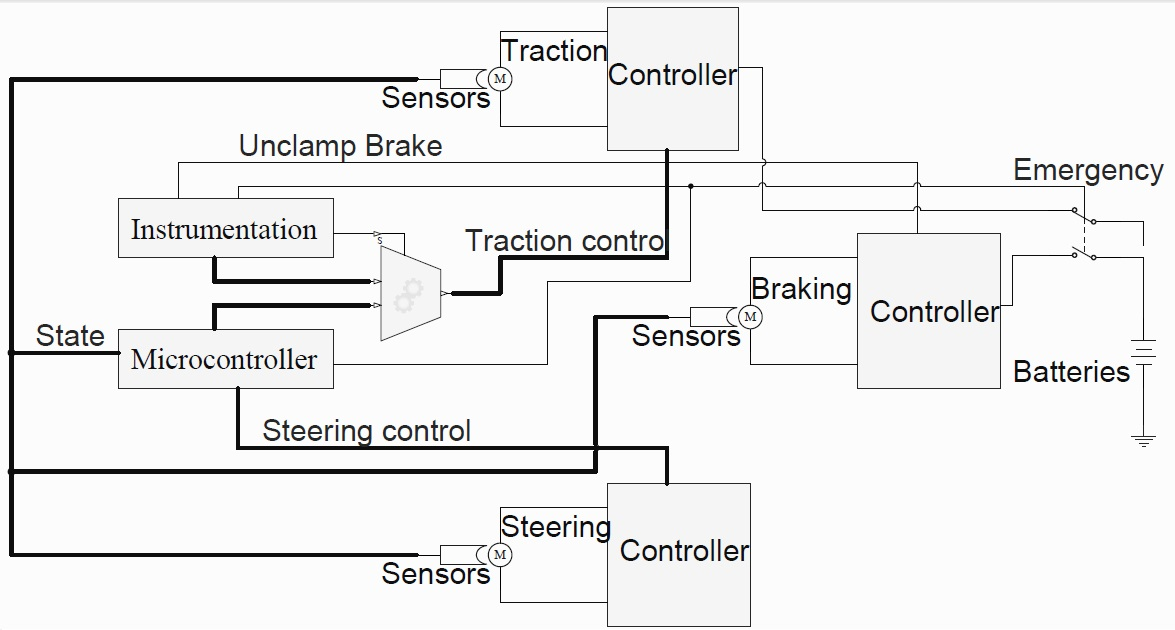
\includegraphics[width=2.5in]{recursos/imagens/block_diagram.jpg}
\caption{Block diagram of the system. Bold connections denote signal buses.}
\label{fig:block_diagram}
\end{figure}

\subsection{Chassis of the ROVIM}

A chassis from a quad motorcycle with internal combustion engine was modified for this application. The old engine and all other unnecessary parts were removed and a wide frame for two platforms was built in its place. In addition, mounting stands for the motors and the sensors were installed. The total kerb weight of the vehicle is just under \SI{250}{\kilo\gram} and its wheel radius measure \SI{23}{\centi\meter} and \SI{28}{\centi\meter} from and rear, respectively.

\subsection{Embedded battery system}

Clever packaging allowed the central lower part of the motorcycle to be used solely for battery placement, in an area free from most accidental interference. However, due to limitations in fabrication methods, it was not possible to fasten them to the chassis nor properly insulate their contacts.

On the lower platform, six \ac{VRLA} batteries were installed in a series connection and provide a maximum of \SI{150}{\ampere} at \SI{12}{\volt} and \SI{72}{\volt} outputs and store \SI{4.05}{\kilo\watt\hour}. Chargers for individual batteries and for the whole group were also acquired.

\subsection{Traction of the ROVIM}

To estimate the power needed to propel the vehicle, a worst-case scenario was designed, where the vehicle is travelling at \SI{3.33}{\kilo\meter\per\hour} in a sandy terrain with a \SI{150}{\kilo\gram} extra load. According to \cite[p. 117]{coefs_atrito}, the typical rolling resistance of car tires on sand is \num{0.3}. At such low speeds, the force resisting vehicle motion can be approximated to the rolling resistance so, from the relation between torque and power,
%
\begin{equation}
P = \omega \cdot T \label{eq:potencia}
\end{equation}
%
where $P$ is the power delivered by the motor, $T$ is the torque on the wheels needed to win motion resistance and $\omega$ is the angular velocity of the wheels, which can be expressed in terms of the linear velocity by:
\begin{equation}
    \omega = \frac{v}{r}% v \cdot \frac{1}{2 \cdot \pi \cdot r} \cdot 2 \cdot \pi
\end{equation}
%
where $v$ is the linear velocity of the vehicle and $r$ is the rear wheel radius. Since the resistive torque can be approximated as the rolling resistance torque, the total torque is:
%
\begin{align} 
    T &\approx T_{a}\\
      &= m \cdot g \cdot \beta \cdot r \label{eq:binario}
\end{align}
%
where $g$ is the gravity acceleration, $\approx \num{10}$, and $\beta$ is the rolling resistance coefficient. Replacing in \eqref{eq:potencia},
%
\begin{align} \label{eq:potencia_vmb}
    P &= v \cdot m \cdot g \cdot b\\
      &= \frac{3.33}{3.6} \cdot 400 \cdot 10 \cdot 0.3\\
      &= \SI{1.1}{\kilo\watt}
\end{align}

Despite the expected power needs, a powerful Lynch type, \SI{16}{\kilo\watt} motor was selected to propel the vehicle that could be placed above the rear fork, freeing up space for the batteries at the center and allowing the modules to be neatly separated. To connect the power to the wheels, a single ratio gearbox was designed and commissioned, allowing reuse of the original sprockets, control over component layout and enabling a higher reduction ratio than commercially available options. The set up of the traction actuator is shown in \figurename~\ref{fig:motor_trc}, and was placed to align the rear axle and the gearbox sprockets.

\begin{figure}[!t]%[bhp]
    \centering
%        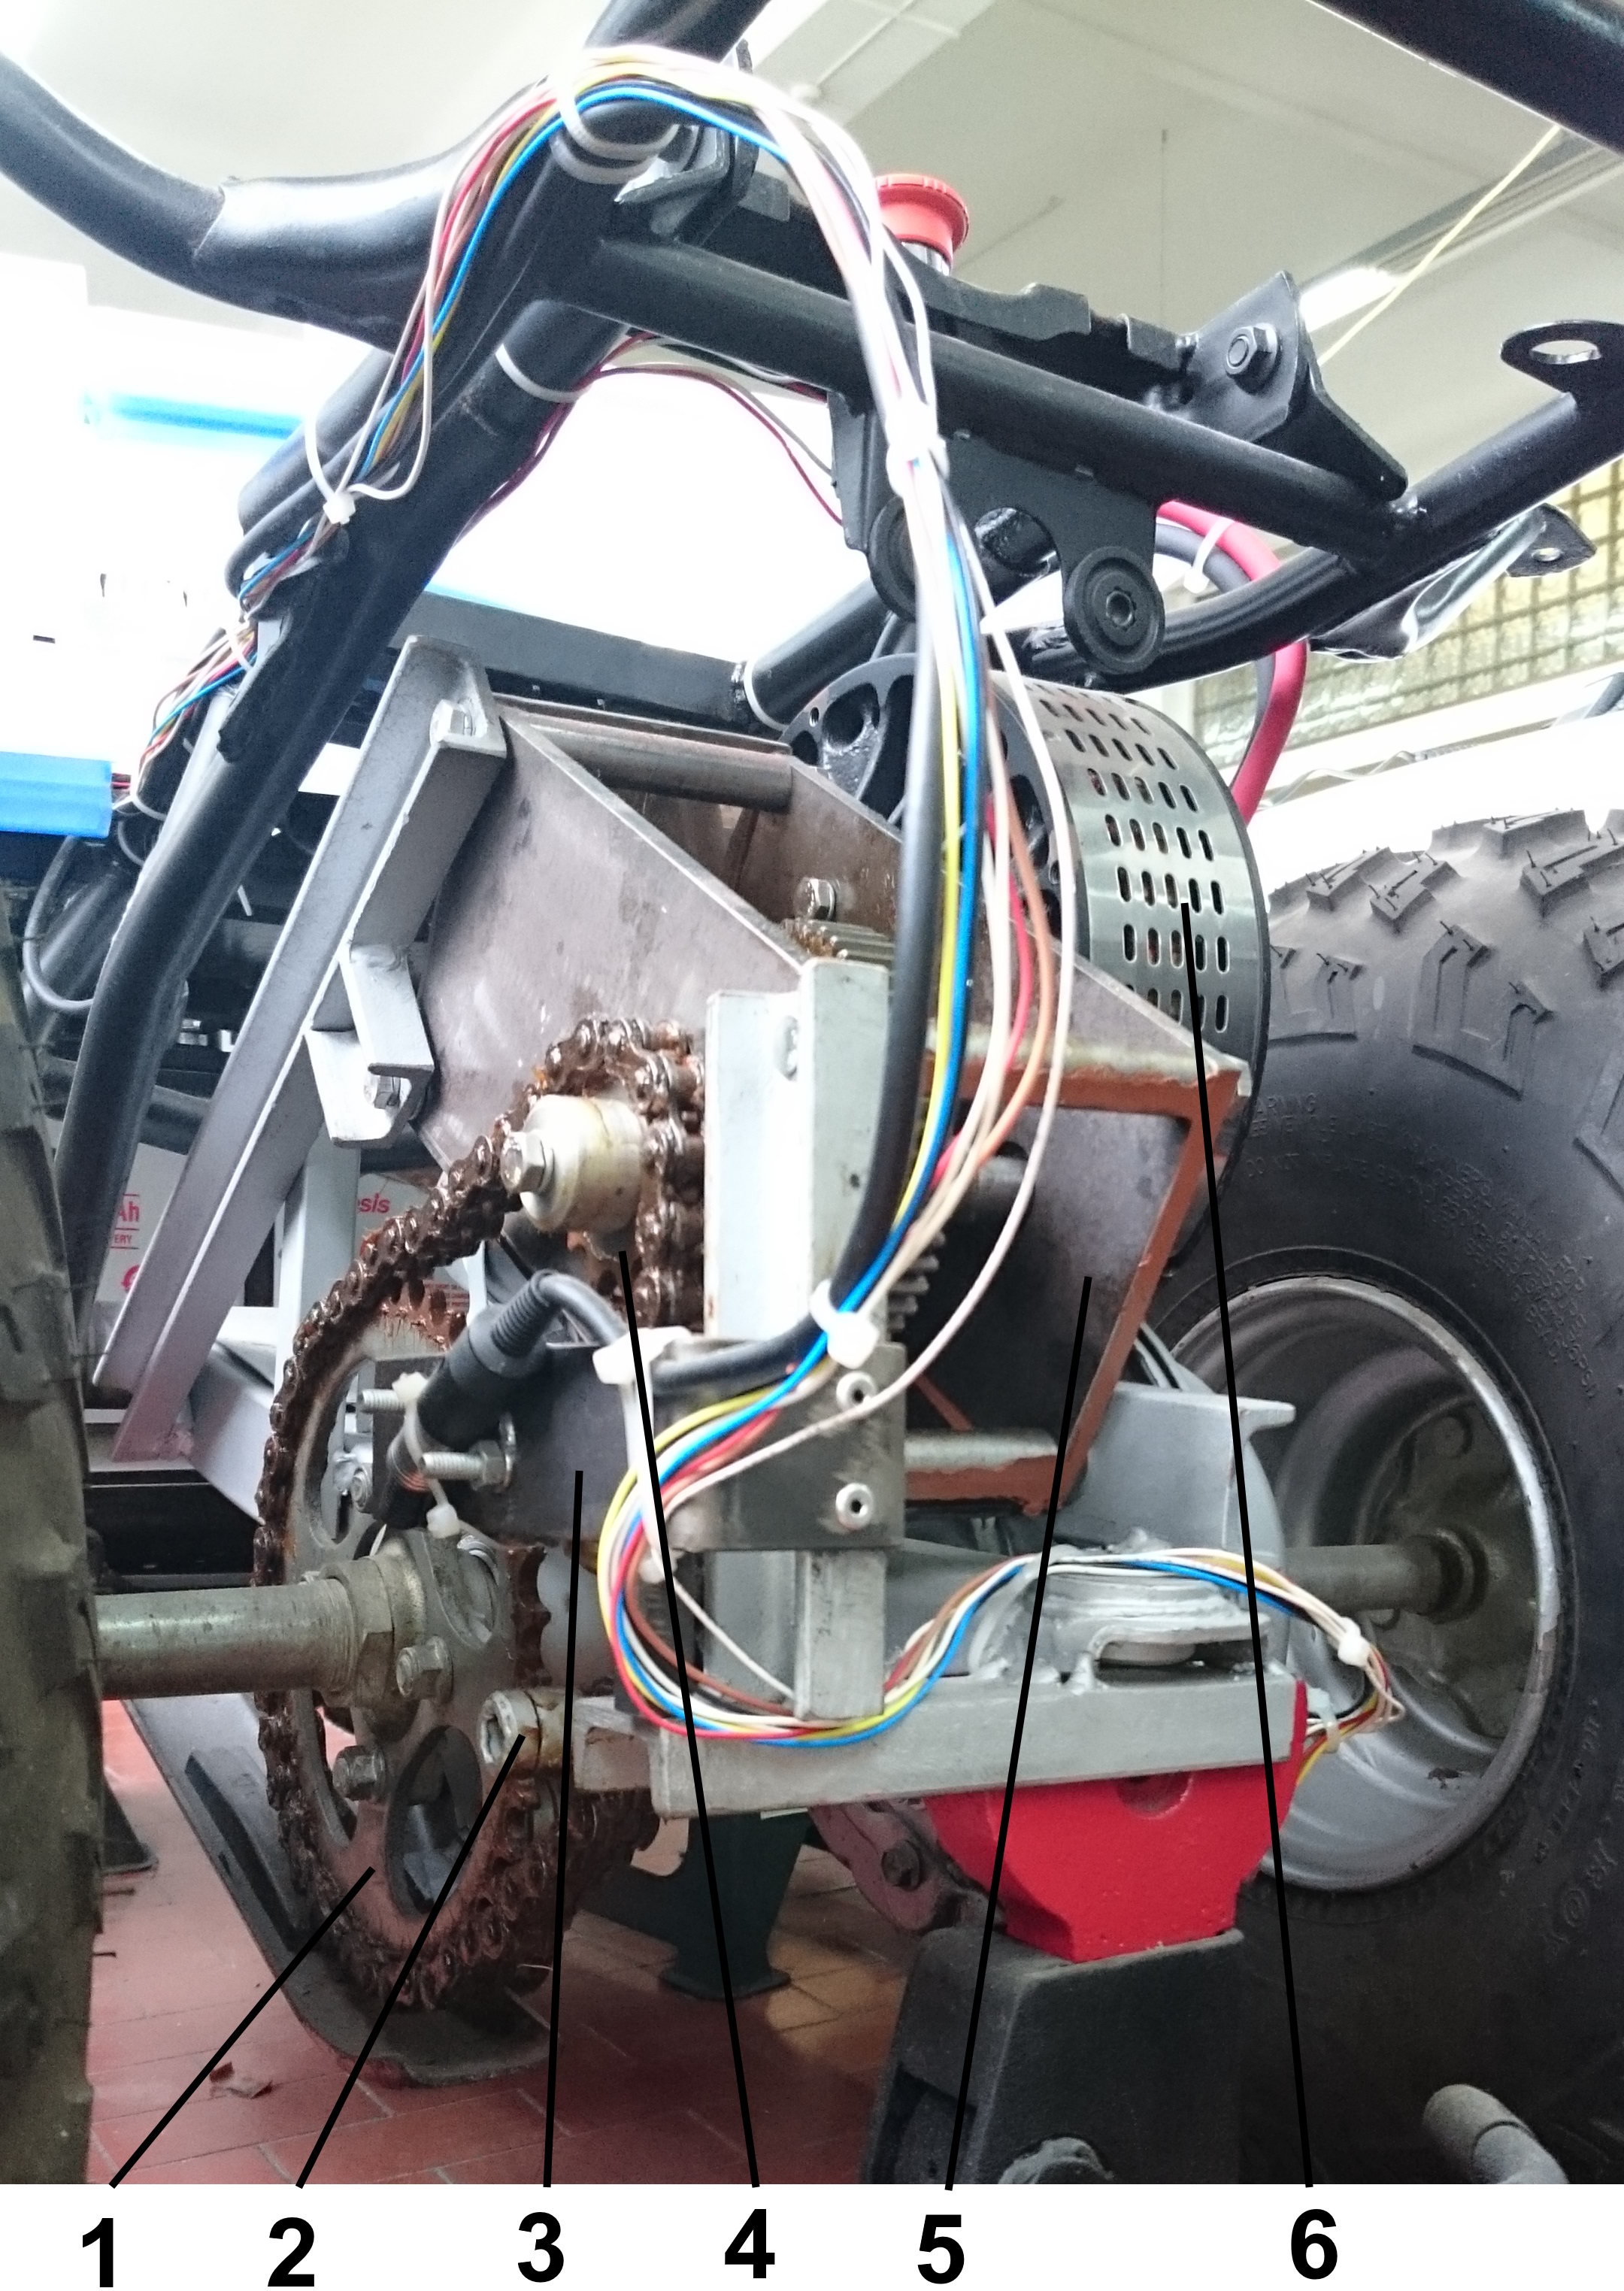
\includegraphics[width=2.5in]{recursos/imagens/motor+redutor.jpg}
%        \caption{Traction motor mount: 1 -- rear axle sprocket; 2 -- chain tensioner; 3 -- sensor mount; 4 -- reductor exit sprocket; 5 -- transmission reductor; 6 -- motor.}
        \subfloat[]{
        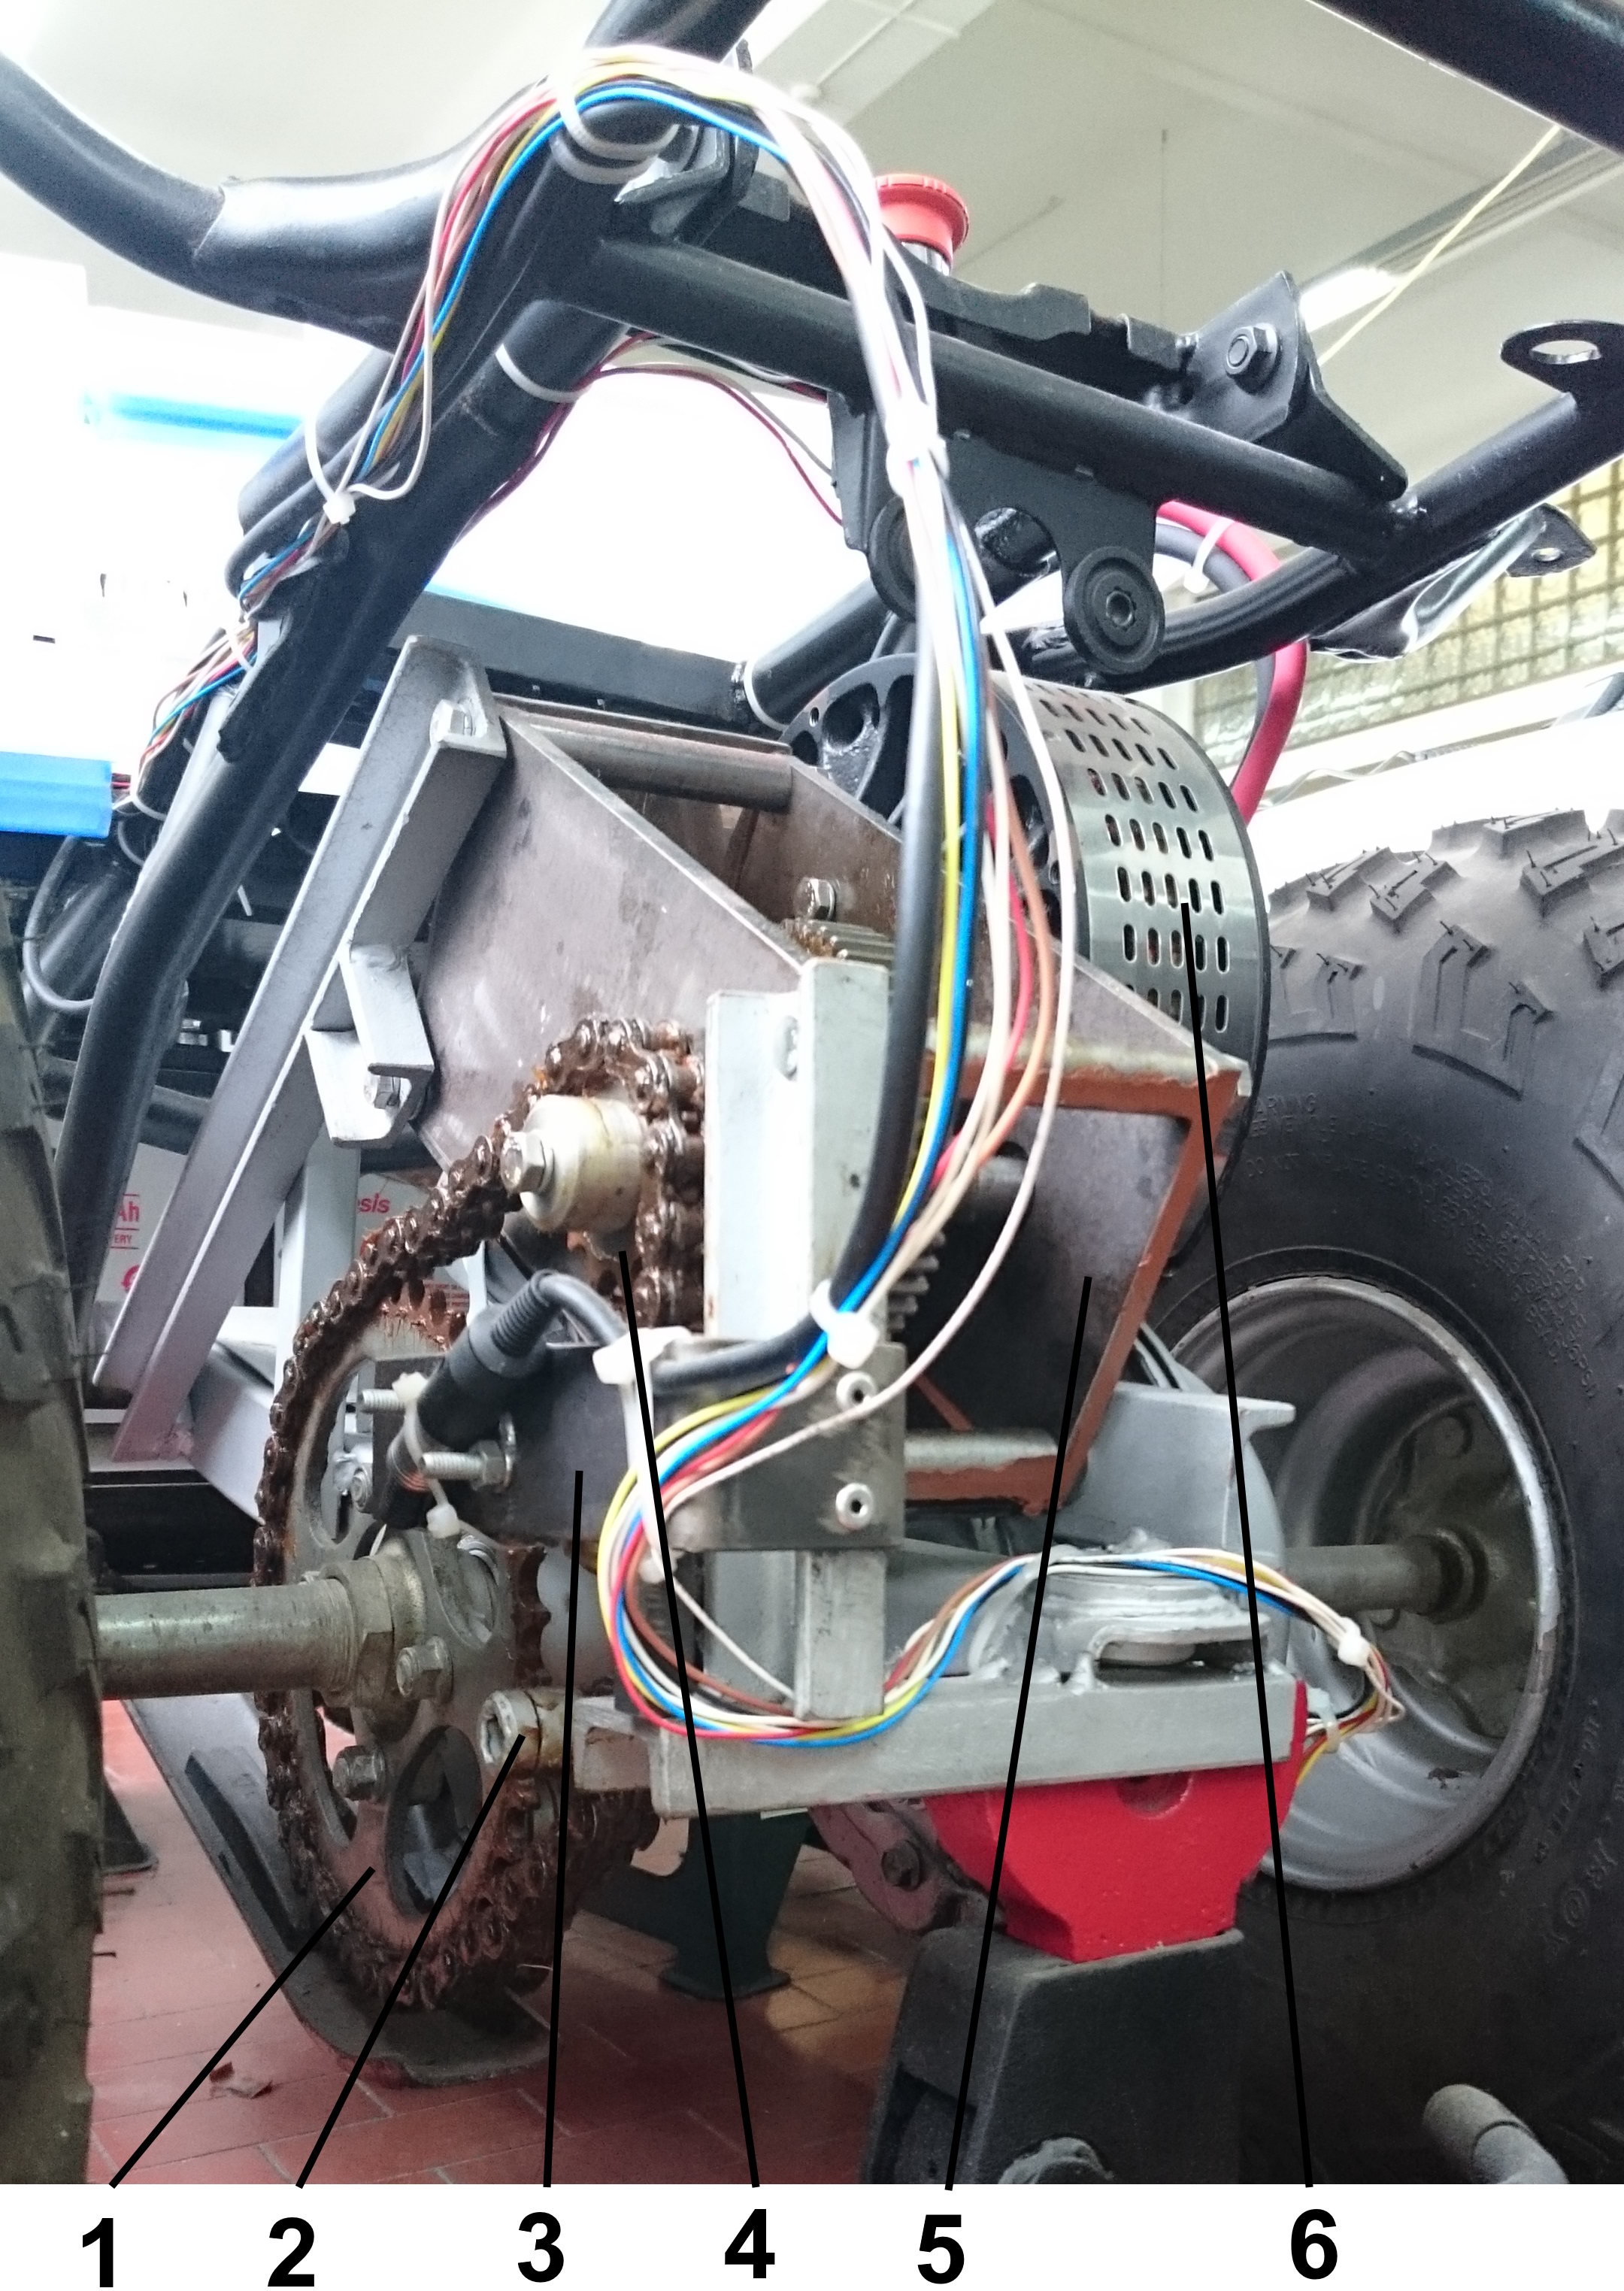
\includegraphics[width=2in]{recursos/imagens/motor+redutor.jpg} 
        \label{fig:motor_trc}}
        %\par\bigskip
        \hfill
        \subfloat[]{
        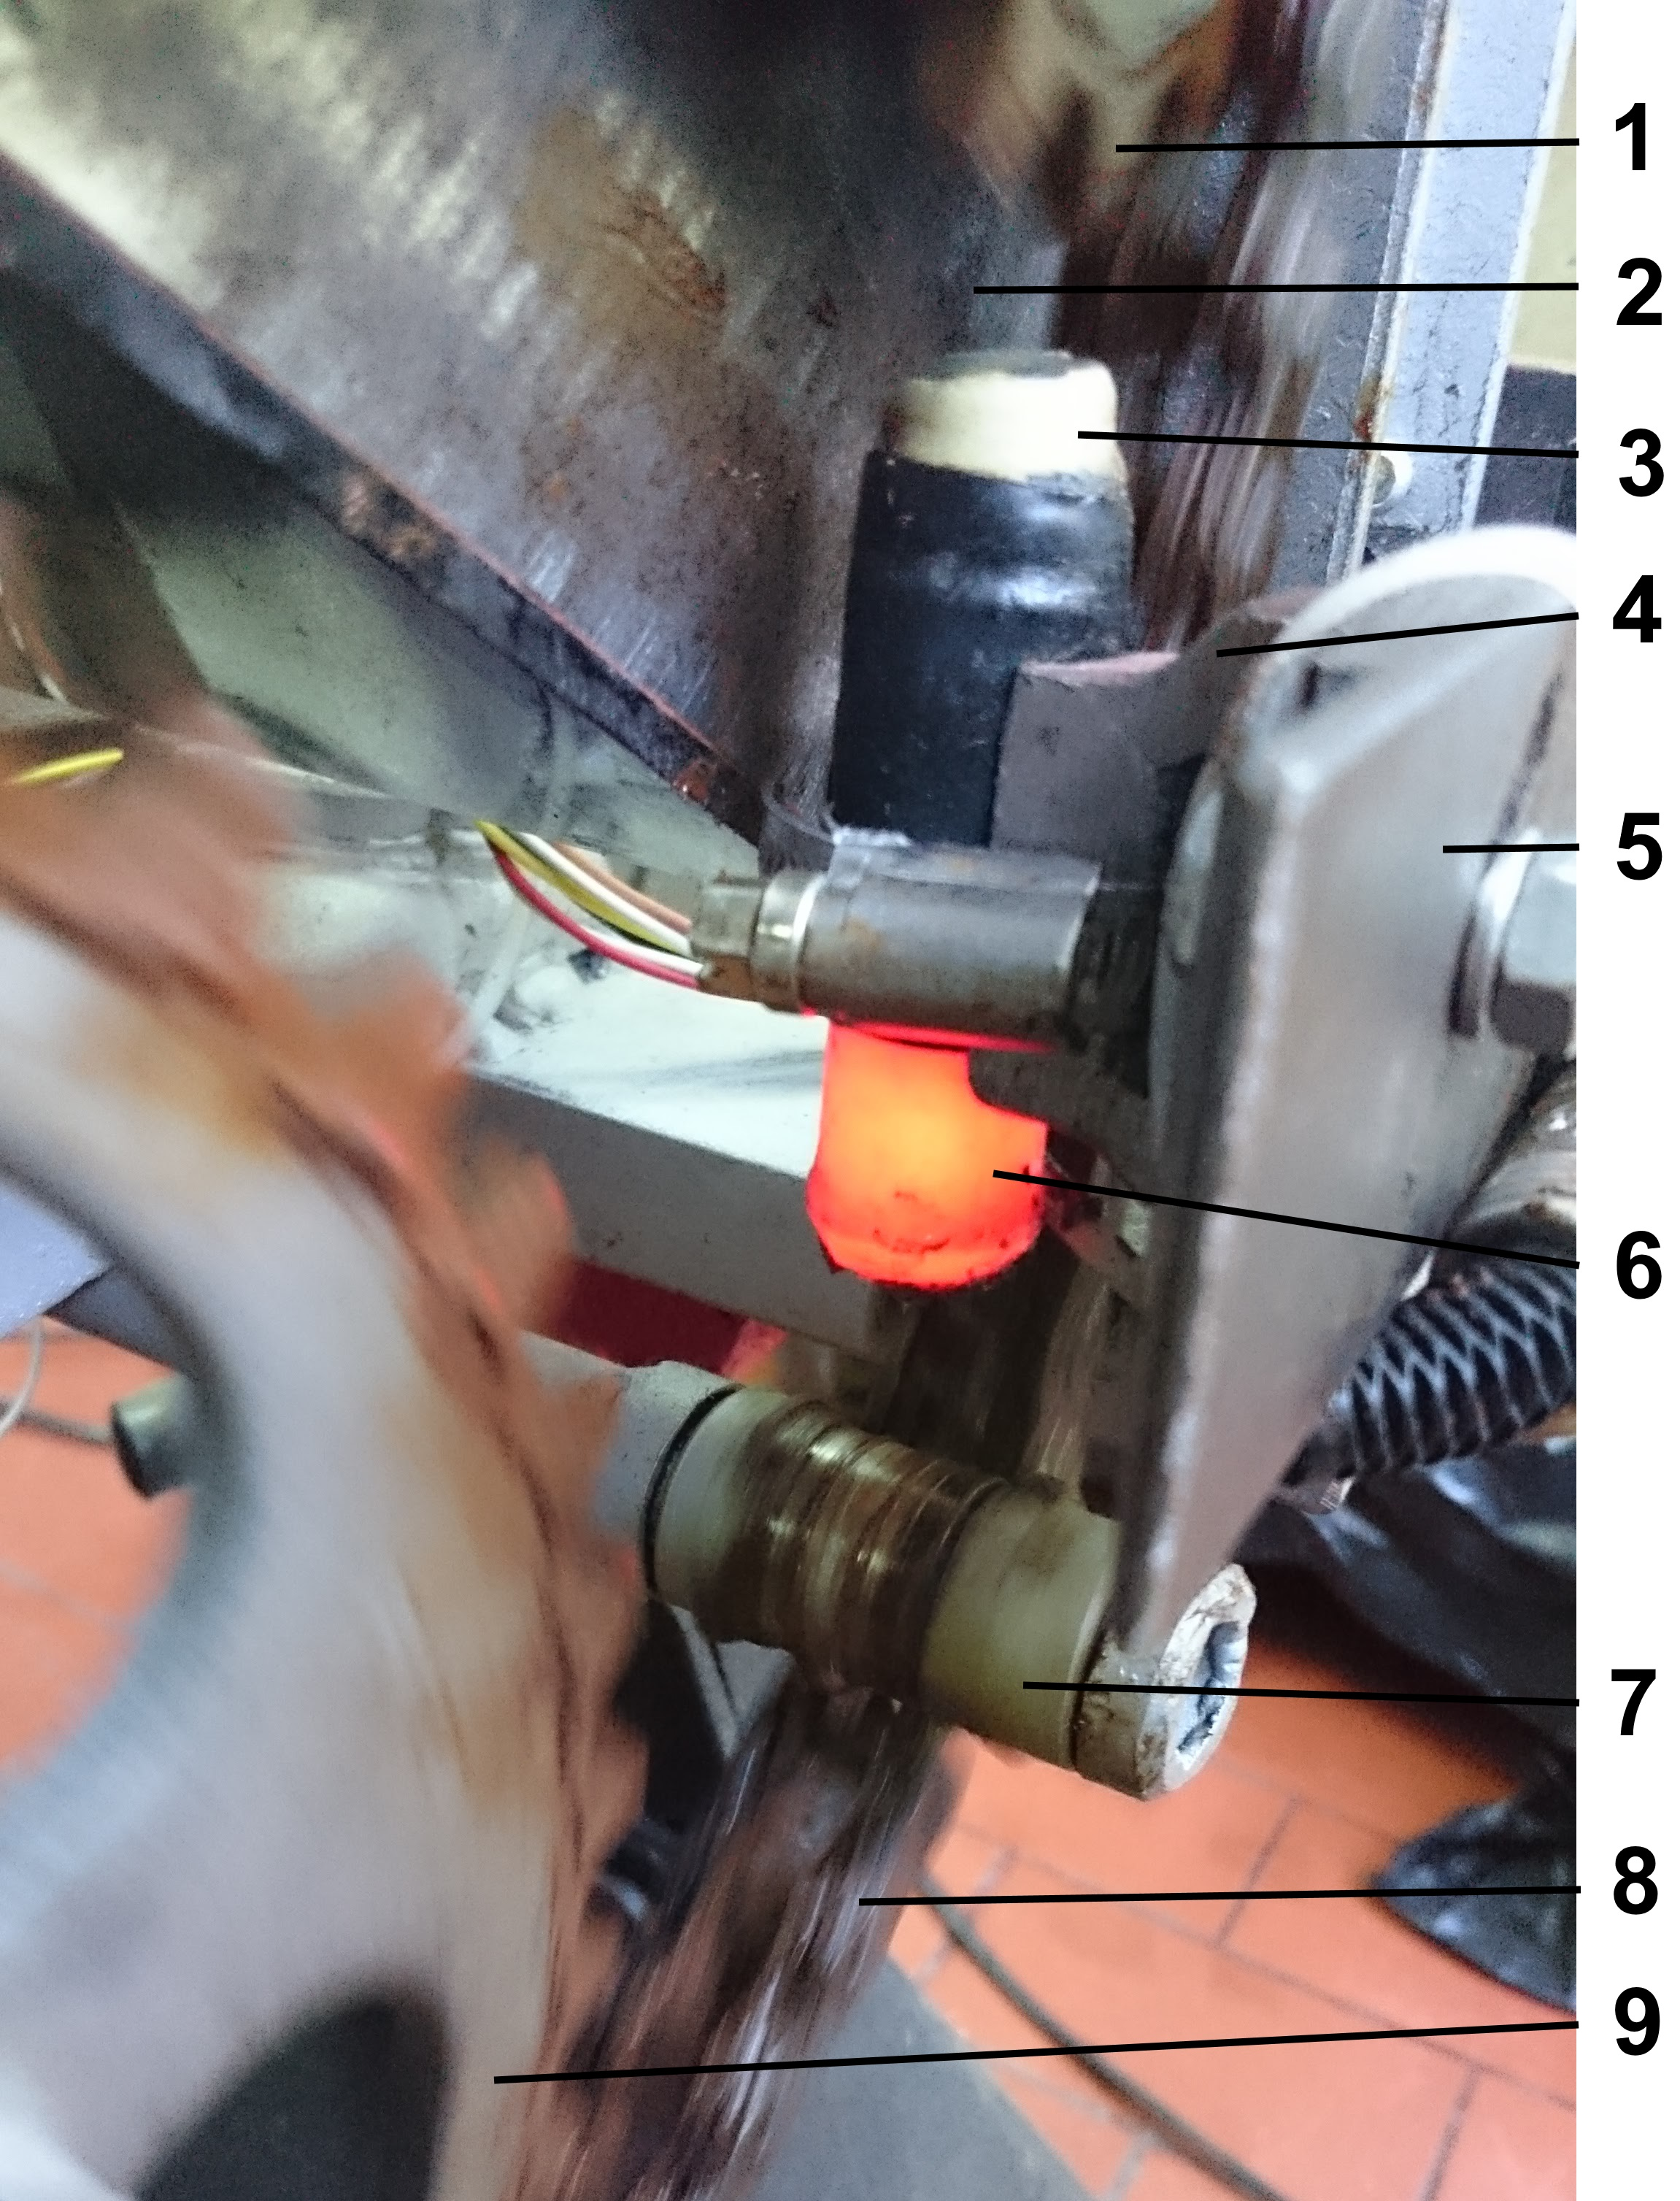
\includegraphics[width=2in]{recursos/imagens/sensor_velocidade.jpg} 
        \label{fig:encoder}}
        \hfill
        \subfloat[]{
        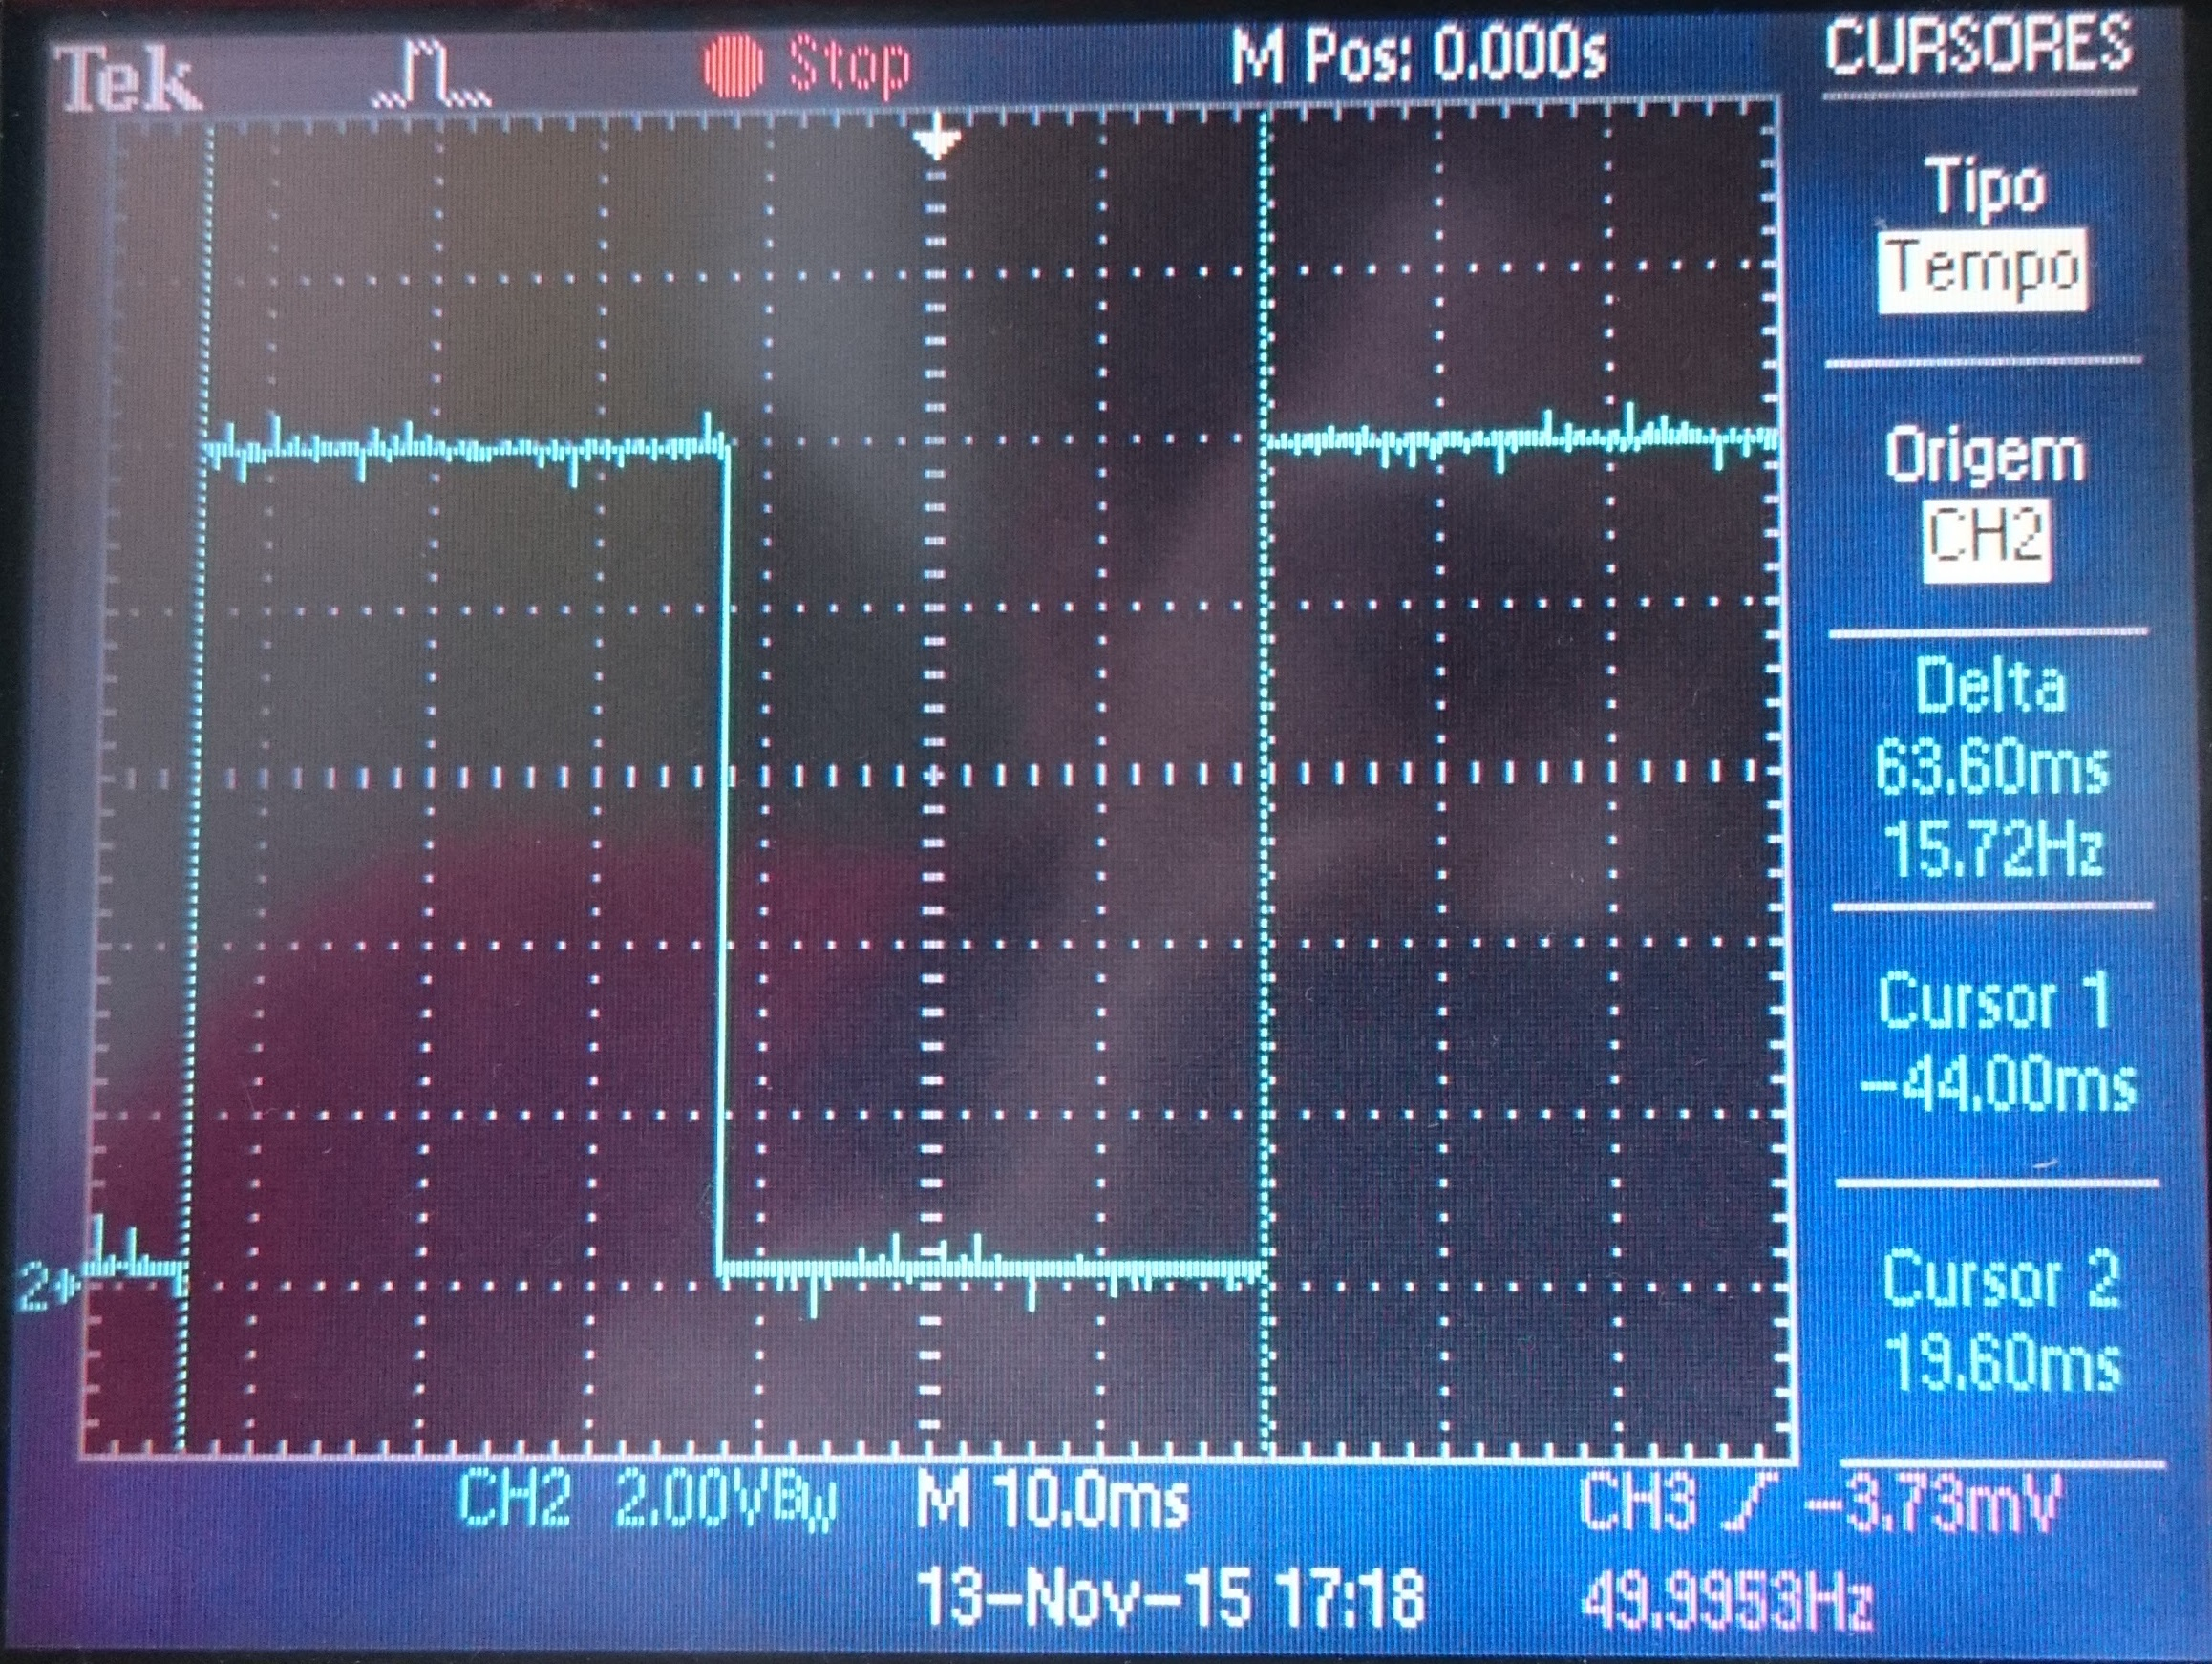
\includegraphics[width=2in]{recursos/imagens/sinal_encoder_2_55kmh.jpg} 
        \label{fig:saida_encoder}}
        \caption[]{ROVIM traction subsystem's sensors and actuators.\\\hspace{\textwidth}a) traction actuator mount: 1 -- rear axle sprocket; 2 -- chain tensioner; 3 -- sensor mount; 4 -- reductor exit sprocket; 5 -- transmission reductor; 6 -- traction motor.\\\hspace{\textwidth}b) speed sensor mount: 1 -- reductor exit sprocket; 2 -- transmission reductor; 3 -- sensor capsule; 4 -- mounting adaptor; 5 -- mounting structure; 6 -- signal light; 7 -- chain tensioner; 8 -- chain; 9 -- rear axle sprocket.\\\hspace{\textwidth}c) sensor readings from a \SI{86}{rpm} mounted gear. Y axis is sensor output voltage at \SI{2}{\volt/div}; X axis is time at \SI{10}{\milli\second/div}.}

\end{figure}

%\begin{figure}[!t]
%\centering
%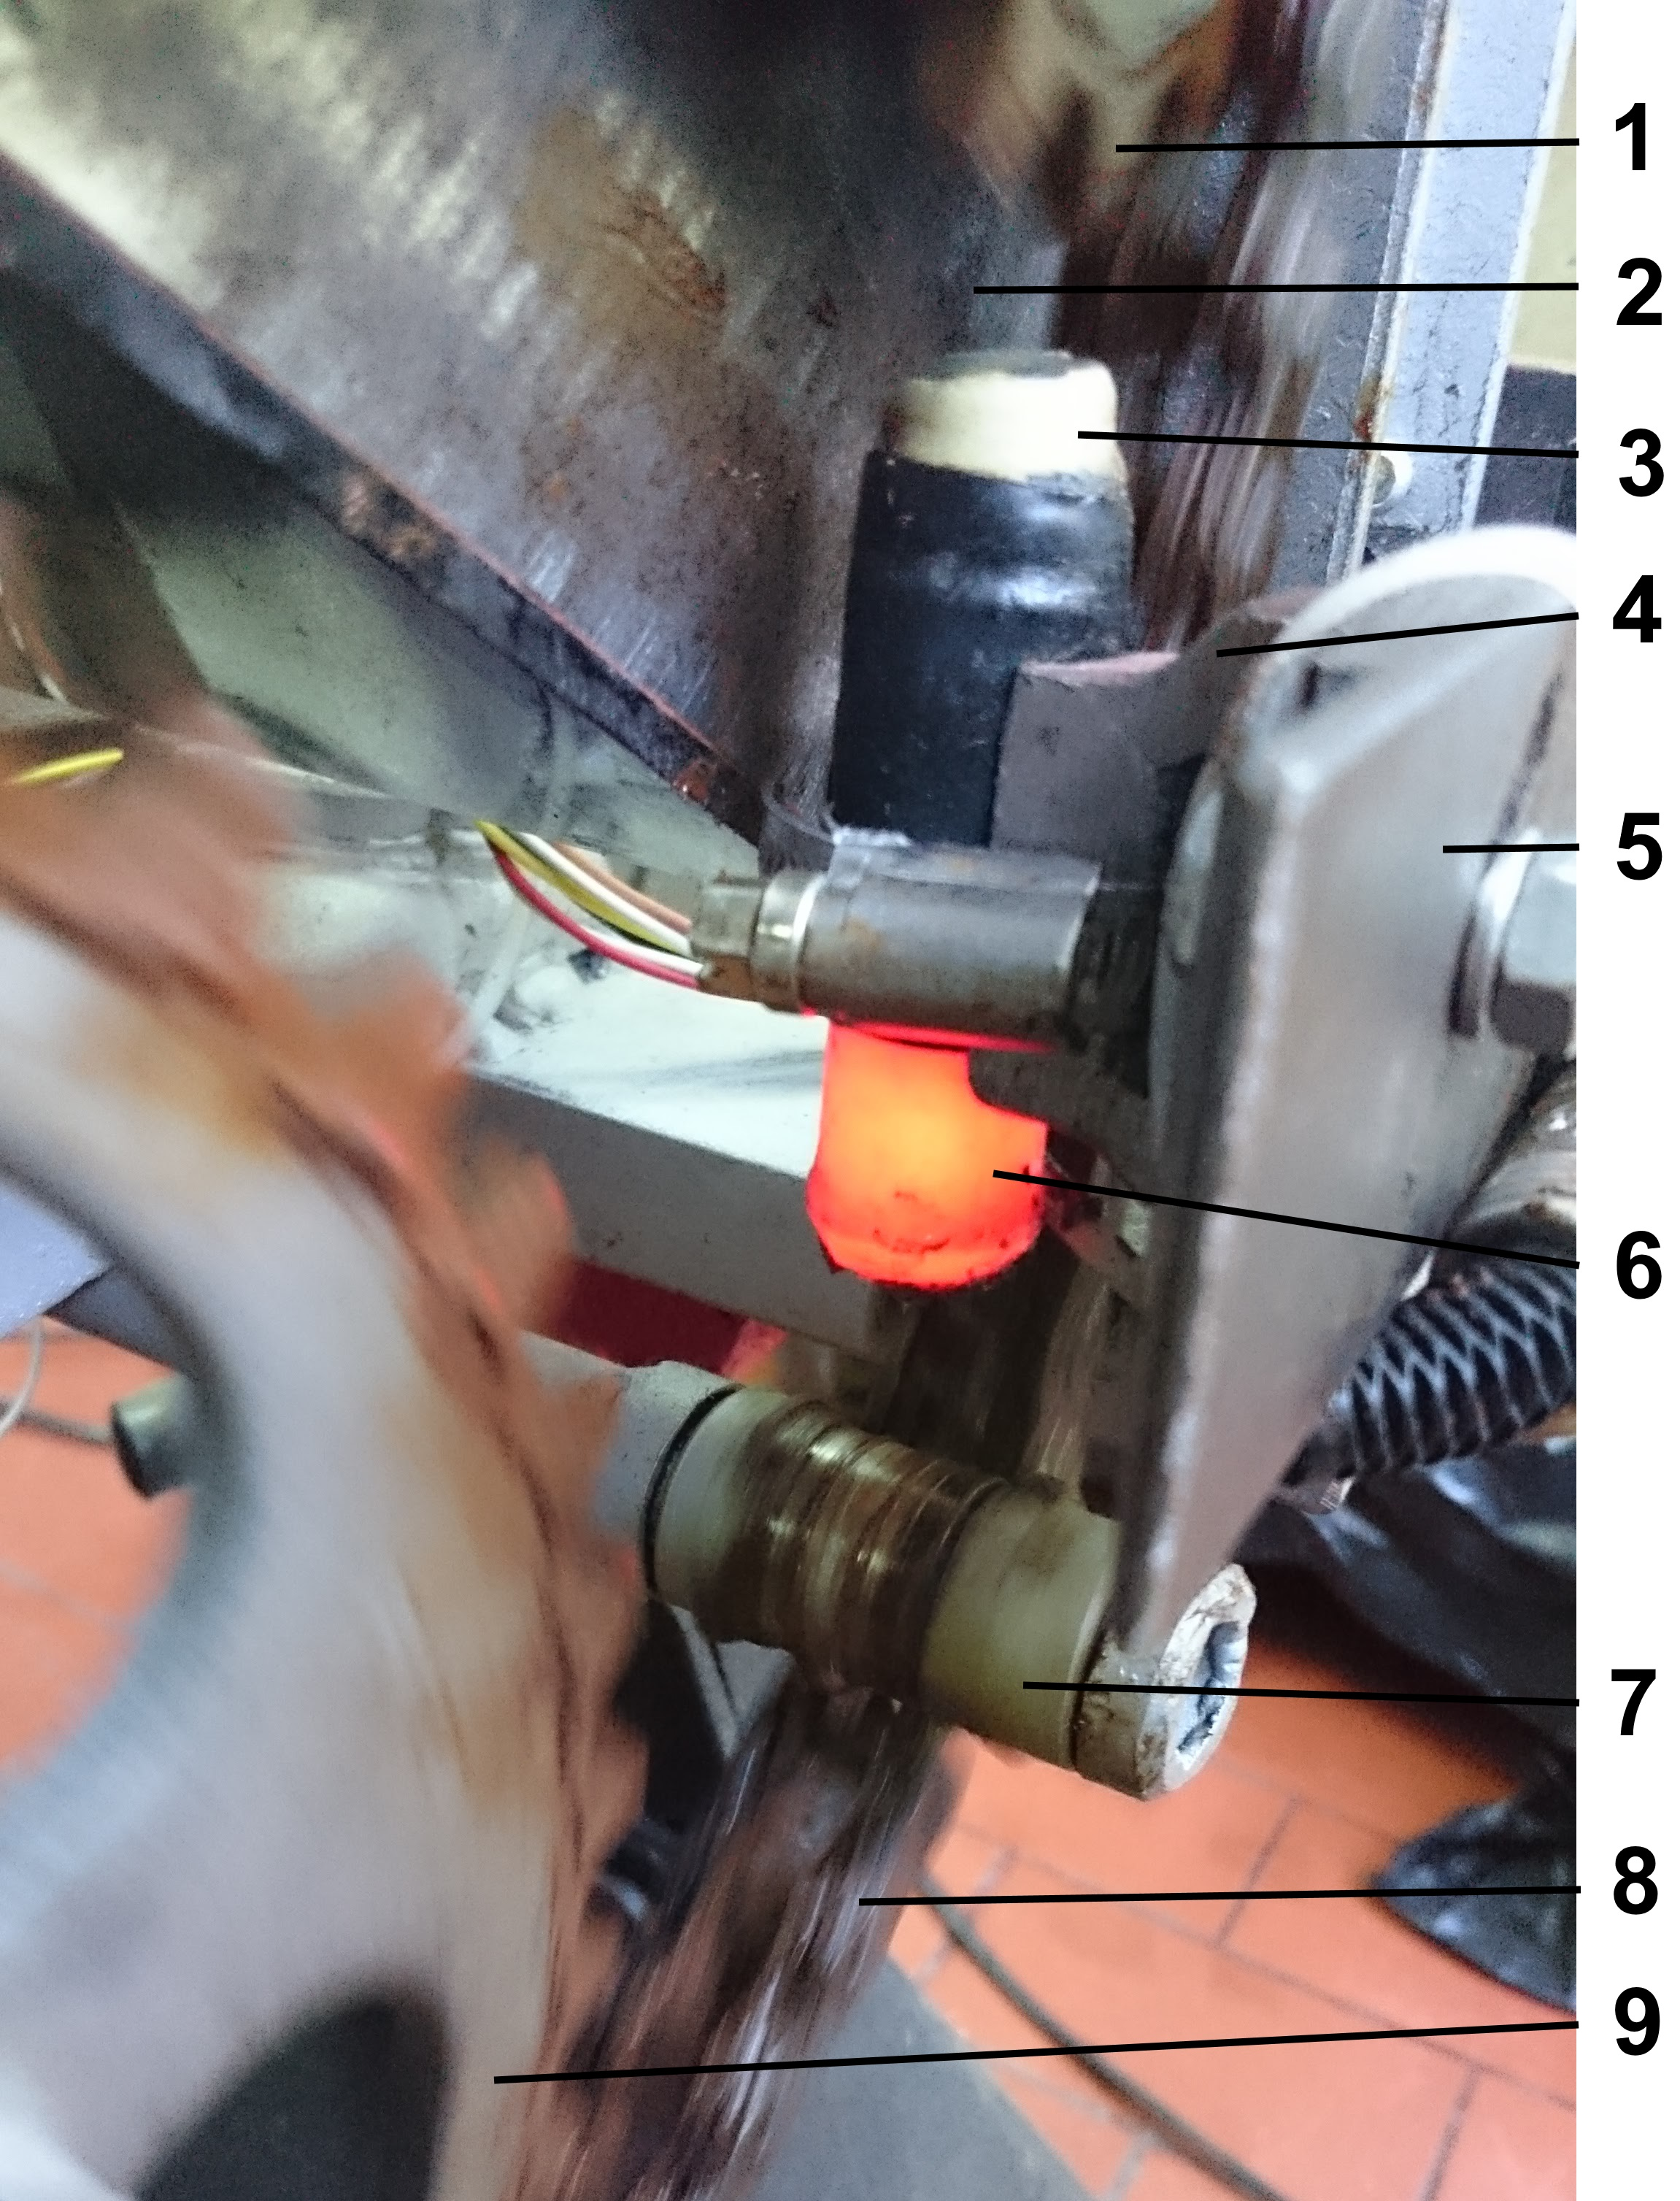
\includegraphics[width=2.5in]{recursos/imagens/sensor_velocidade.jpg}
%\caption{Sensor mount:}% 1 -- reductor exit sprocket; 2 -- transmission reductor; 3 -- sensor capsule; 4 -- mounting adaptor; 5 -- signal light; 7 -- chain tensionner; 8 -- chain; 9 -- rear axle sprocket.}
%\label{fig:encoder}
%\end{figure}

A four quadrant permanent magnet \ac{DC} motor controller recommended by the motor manufacturer was acquired in a easy assemble kit and initially wired according to \cite[p. 15]{datasheet_PMT835M} to achieve manual driving functionality and evaluate the work plan at an intermediate stage. After that, additions discussed in \ref{ssec:integracao} were made to achieve autonomous driving capabilities.

\subsubsection{Traction speed encoder}

To measure the vehicle speed, a variable reluctance sensor was built and attached to the actuator set--up, near the gearbox exit sprocket, as shown in \figurename~\ref{fig:encoder}. It consists of a small permanent magnet with a ferromagnetic pole attached and a copper coil wired around the pole and connected to a \ac{PCB} signal conditioning circuit. When the pole side of the sensor is placed near a metallic rotating teethed gear, an alternating voltage is induced in the coil, which is first rectified and amplified by a half wave precision rectifier, and then converted into a binary signal whose frequency is proportional to the gear speed, by a comparator with hysteresis. A \ac{LED} at the circuit exit provides visual confirmation of motion detection. Sensor consumption was measured at \SI{300}{\micro\ampere} at idle and \SI{15}{\milli\ampere} on high frequency operation, and its performance on the final mount at different speeds is shown in \figurename~\ref{fig:saida_encoder}.

\subsection{Braking mechanisms of the ROVIM}

The vehicle can reduce speed in three different ways: through the original front brake lever, the traction motor controller's regenerative braking feature and the rear drum brake. The first two are used in manual and autonomous driving modes, respectively to reduce the vehicle's speed during normal operation. The rear brake performs emergency braking, and is actuated by a servomotor dimensioned empirically, placed above the rear fork and connected to the brake lever by a worm screw that screws a pivot attached to the lever. The set--up of the rear brake actuator is shown in \figurename~\ref{fig:motor_trv}. Due to the unidirectional torque transmission characteristics of the screw and pivot set--up, the brake stays locked even when it is not being powered.

Instead of an electronic controller, it is controlled by more transient resilient relays and mechanical switches, arranged in two circuits: a safety mechanism that triggers braking, detailed in \ref{ssec:halt} and a power connection circuit. The brake is connected to the batteries by a polarity switching relay, and the braking polarity leg of the circuit (on by default) is passed through the safety mechanism. The power is fed through end of travel switches mounted to detect each side of the lever travel end, that open the circuit when reached. The set--up of the end of travel mounts is shown in \figurename~\ref{fig:fdc_trv}.

The polarity can be inverted to unlock the brake by a user activated pressure button or a microcontroller signal, that was not connected at this stage.

\begin{figure}[!t]%[bhp]
    \centering
        \subfloat[]{
        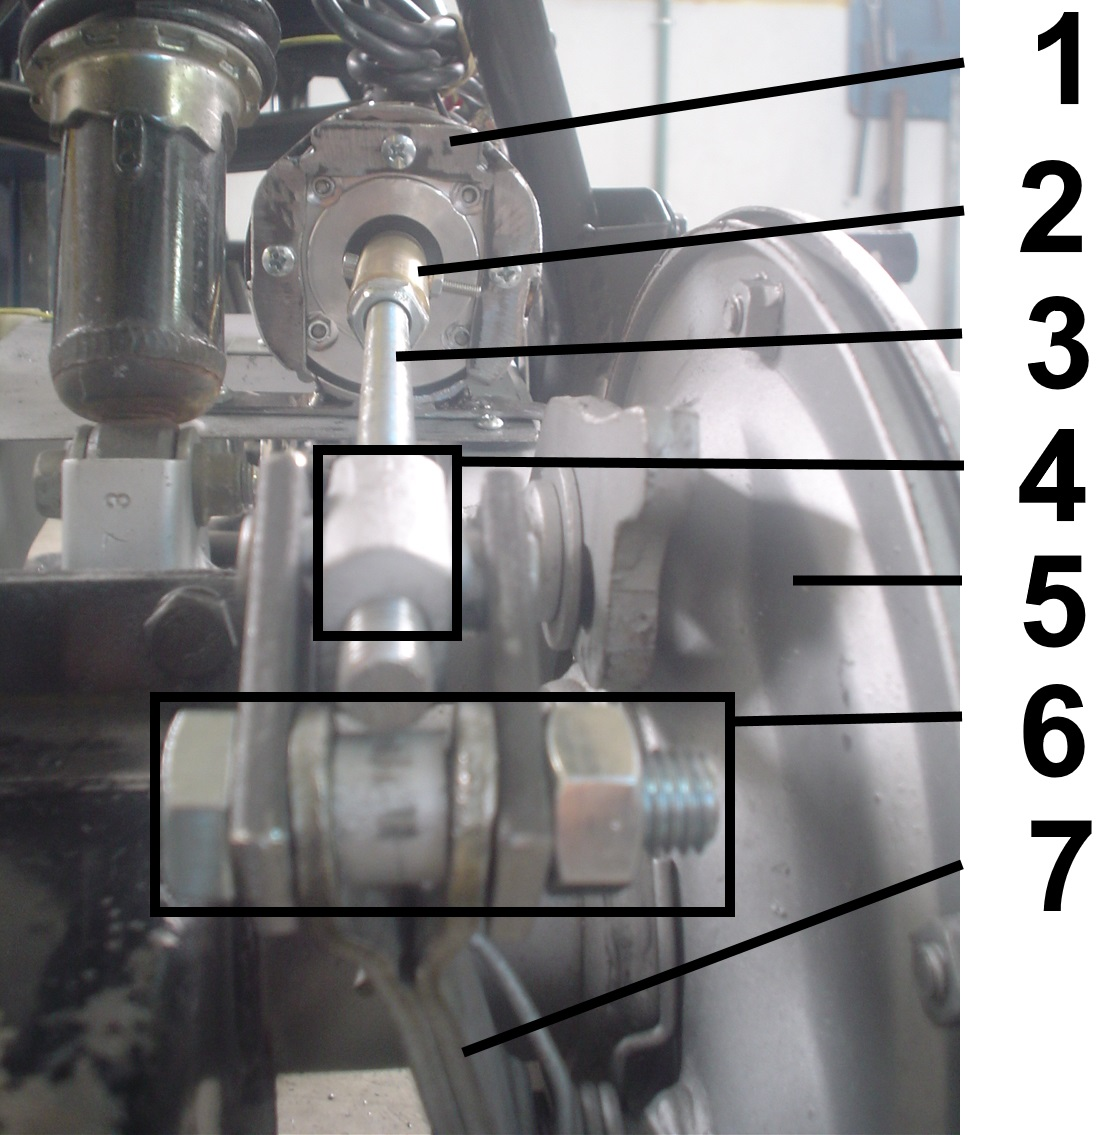
\includegraphics[width=2in]{recursos/imagens/trv_montagem.jpg} 
        \label{fig:motor_trv}}
        %\par\bigskip
        \hfill
        \subfloat[]{
        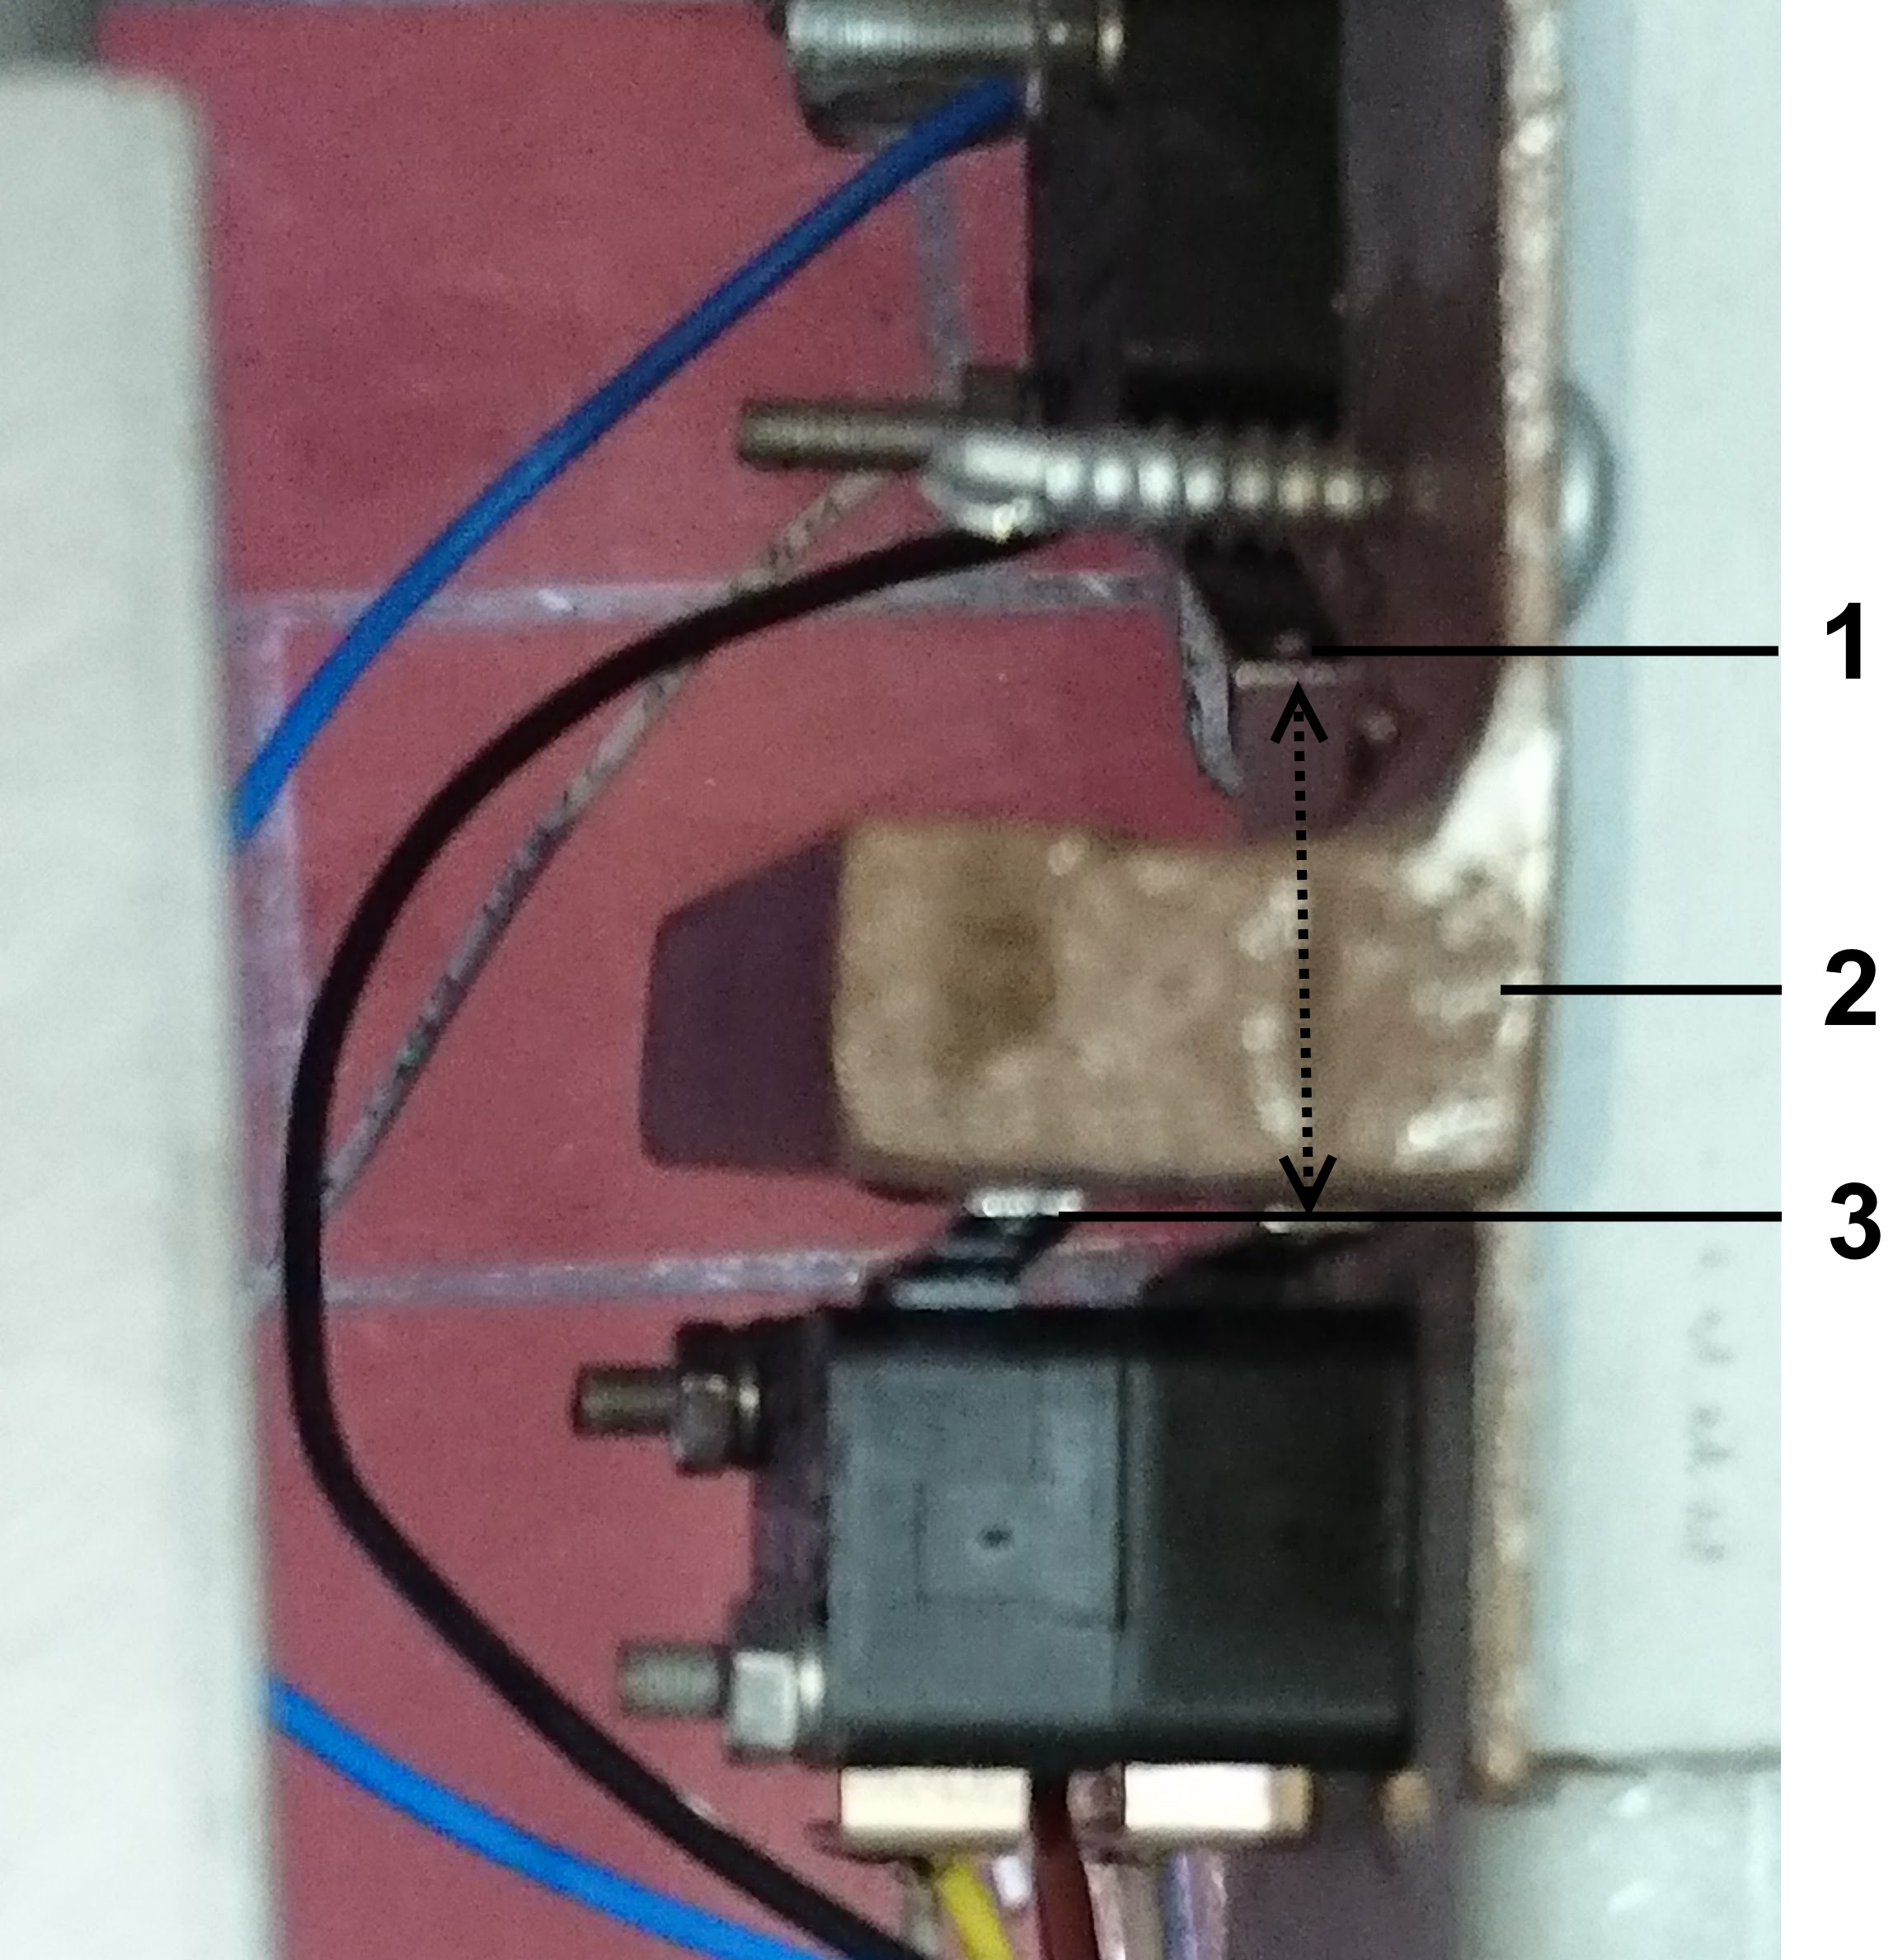
\includegraphics[width=2in]{recursos/imagens/trv_fc_destravado.jpg} 
        \label{fig:fdc_trv}}
        \caption[]{ROVIM braking subsystem's sensors and actuators.\\\hspace{\textwidth}a) brake actuator mount: 1 -- frontal motor fastener; 2 -- shaft adaptor; 3 -- worm screw; 4 -- brake pivot; 5 -- brake drum; 6 -- pivot's brake lever fastener; 7 -- brake lever.\\\hspace{\textwidth}b) brake sensors mount with brake unlocked: 1 -- lock side end of travel switch lever; 2 -- lever travelling jointly with the brake lever that triggers the switches; 3 -- unlock side end of travel switch lever. The dotted arrow denotes the travel of 2.}
\end{figure}

\subsection{Steering system of the ROVIM}

The vehicle turns the wheels through a steering column that can be actuated by the original handlebar of the chassis in manual driving mode, or through an electromechanical actuator in autonomous mode. In order to estimate the size of the steering actuator to use, the  minimum force required at the tip of the handlebar to turn it from the center position was measured with the vehicle immobilized in a tiled surface. With \SI{25}{\newton\meter} the handlebar moved until about \SI{80}{\%} of tis course, from which point a \SI{30}{\newton\meter} force was needed to bring it to its end. The torque applied in this situation can be calculated from:
%
\begin{align}
    T &= F \cdot a\\
        &= 30 \cdot 0.41\\
        &= \SI{12.3}{\newton\meter}
\end{align}
%
where $F$ is the force applied at the tip of the handlebar and $a$ is the handlebar's radius, measured at \SI{0.41}{\meter}. The steering's angular motion range was also measured, at \SI{88.8}{\degree}. Having an Ackerman steering geometry, that is designed for the wheels to turn without slip, the torque needed to run the vehicle in motion can be approximated to its rolling resistance torque. Replacing in \eqref{eq:binario} for the worst case scenario used to estimate the traction actuator:
%
\begin{align}
    T &=400 \cdot 10 \cdot 0.3 \cdot 0.23\\
      &=\SI{273}{\newton\meter}
\end{align}
%
In both the measured and estimated case, the turning torque depends on the friction between the tires and the floor. Since a military vehicle is expected to be rugged enough to drive through a multitude of terrains, the controller of the actuator needs to maintain performance across a wide range of changing conditions.

The actuator employed consists of a servomotor connected to a compact worm drive gearbox that drives the steering column through a dented belt connecting two dented pulleys, attached to the gearbox's output shaft and the steering column, totalling a reduction ratio of \num{98} and allowing a maximum torque of \SI{133.2}{\newton\meter} to be deployed on the steering column. Even though it is smaller than the worst case scenario needs, it was deemed enough and allowed a nimbler actuator to be chosen and mounter lower in the chassis, freeing up area for future expansion needs. The set--up of the steering actuator is shown in \figurename~\ref{fig:motor_dir}. The motor is driven by an off--the--shelf H bridge power converter designed for robotic applications, in turn controlled through a compatible interface with the microcontroller.

\begin{figure}[!t]%[bhp]
    \centering
        \subfloat[]{
        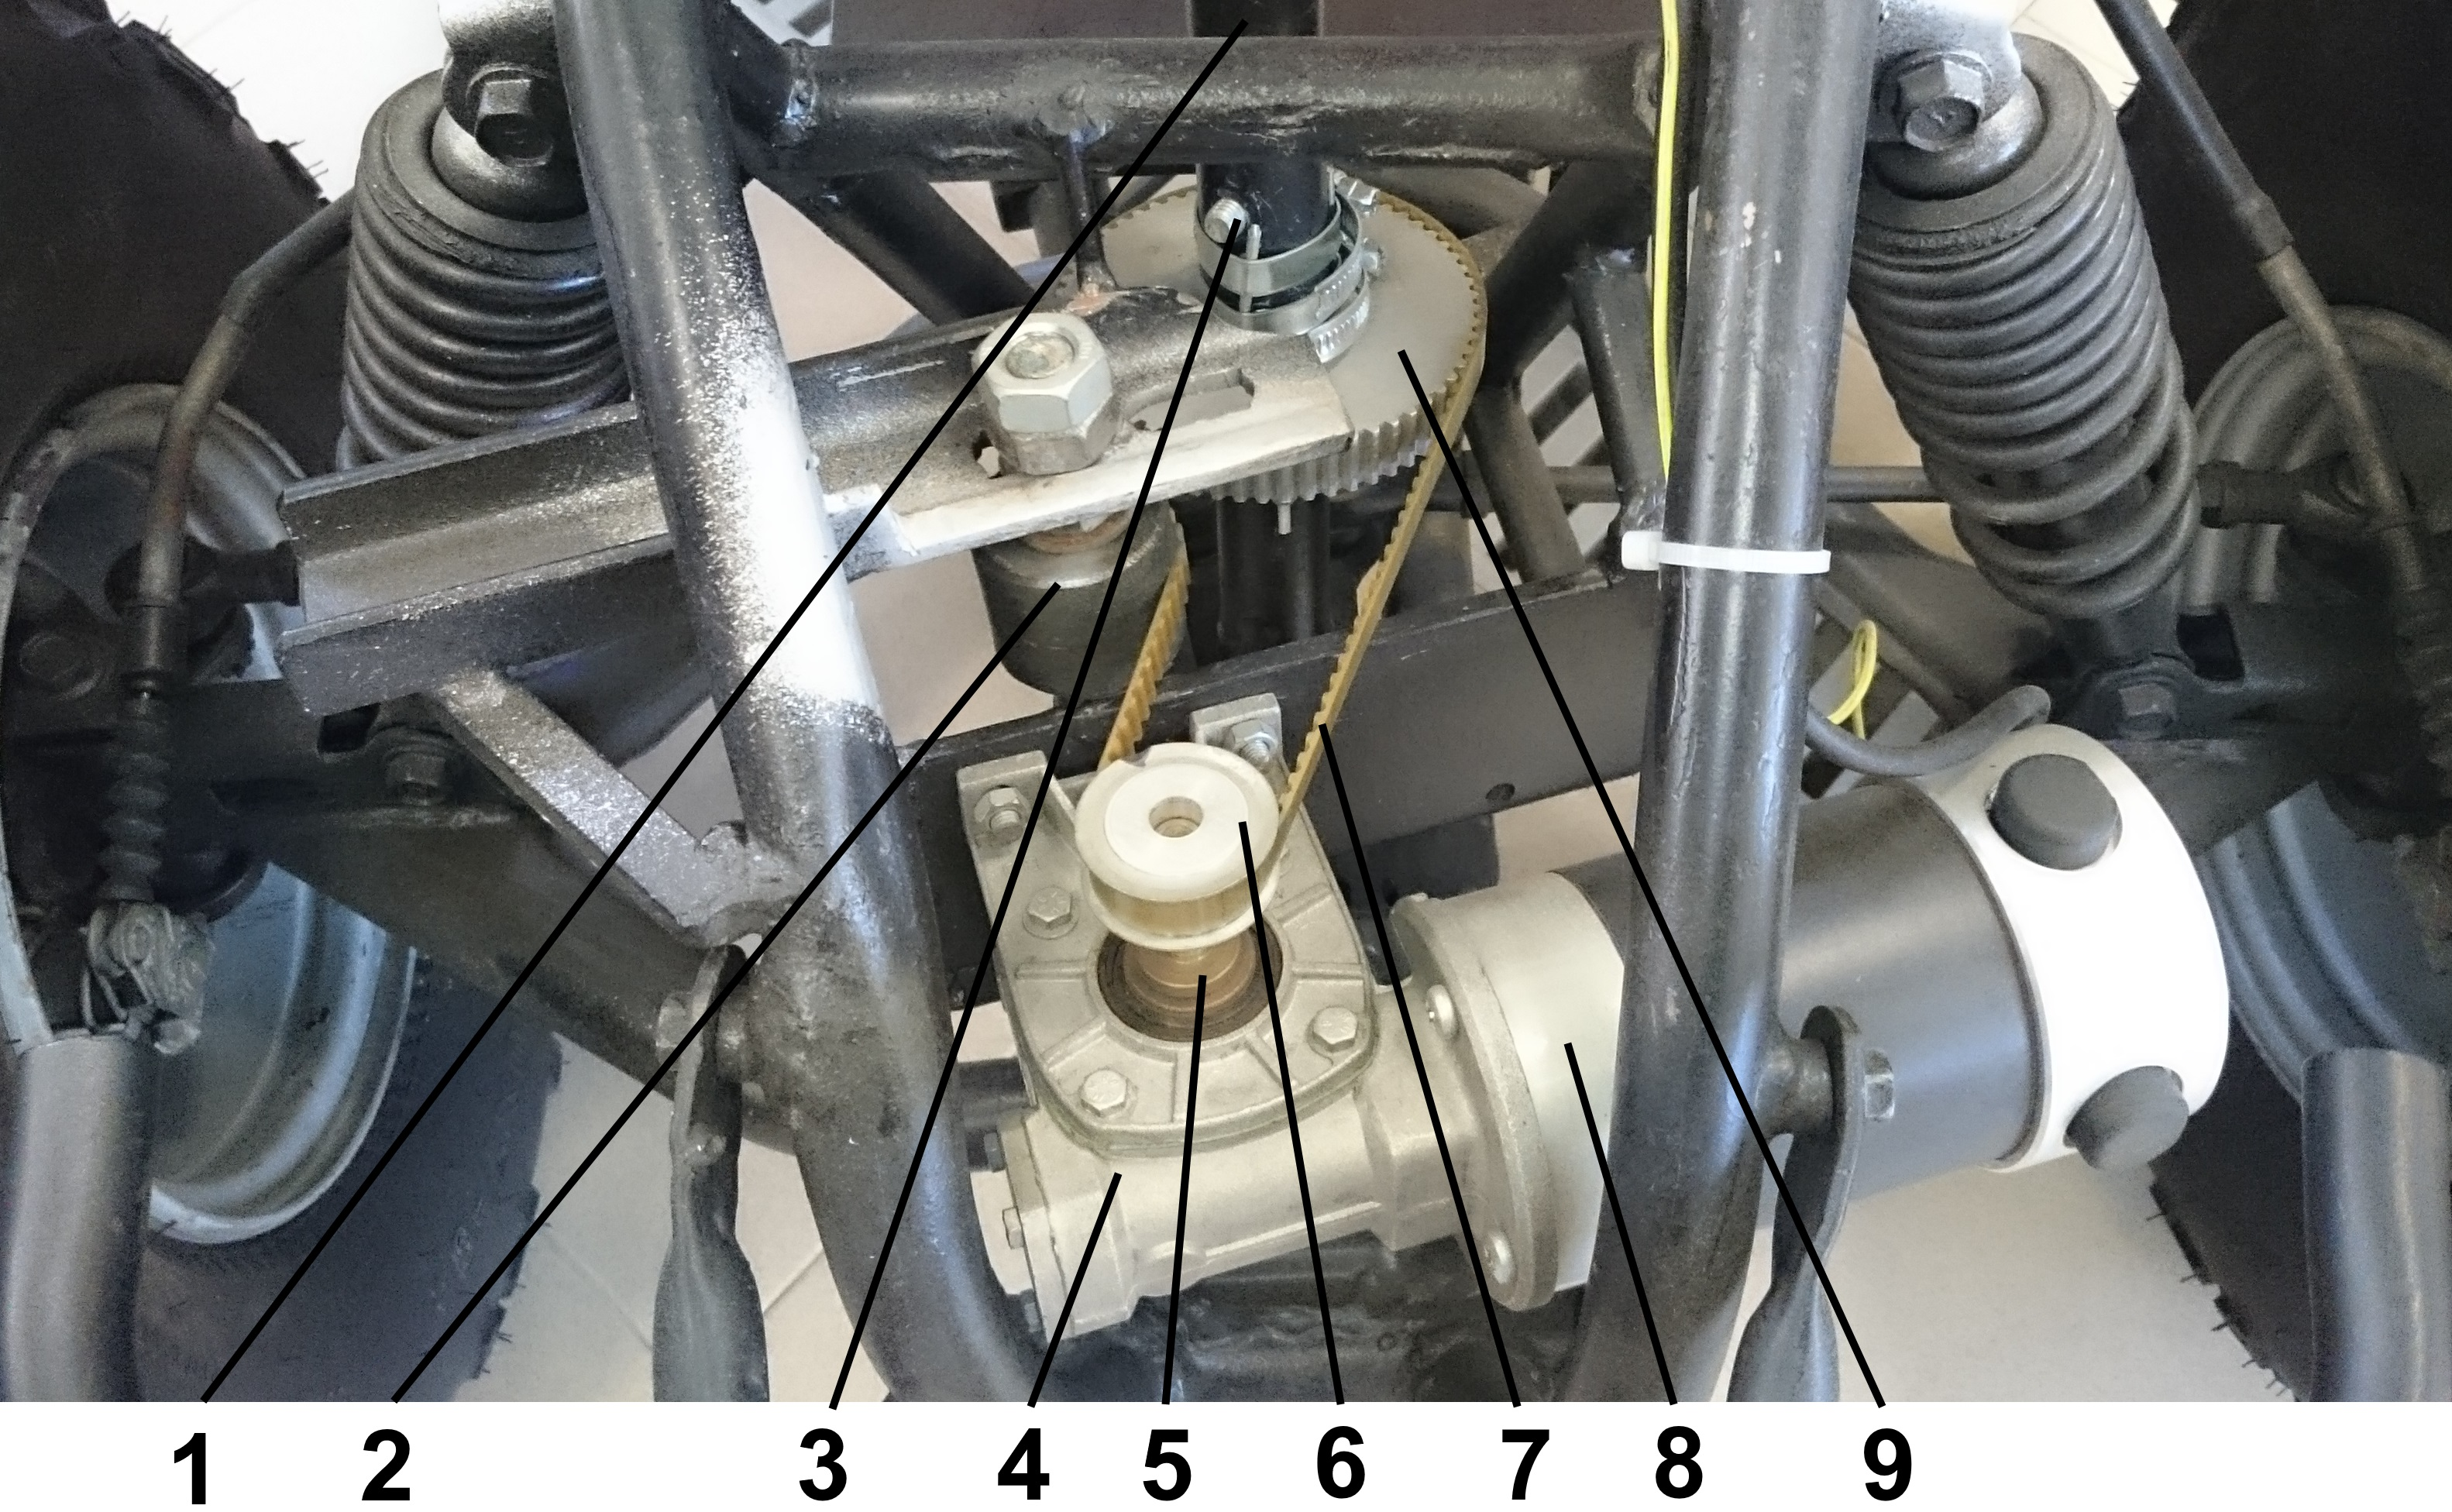
\includegraphics[width=2in]{recursos/imagens/atuador_direcao.jpg} 
        \label{fig:motor_dir}}
        %\par\bigskip
        \hfill
        \subfloat[]{
        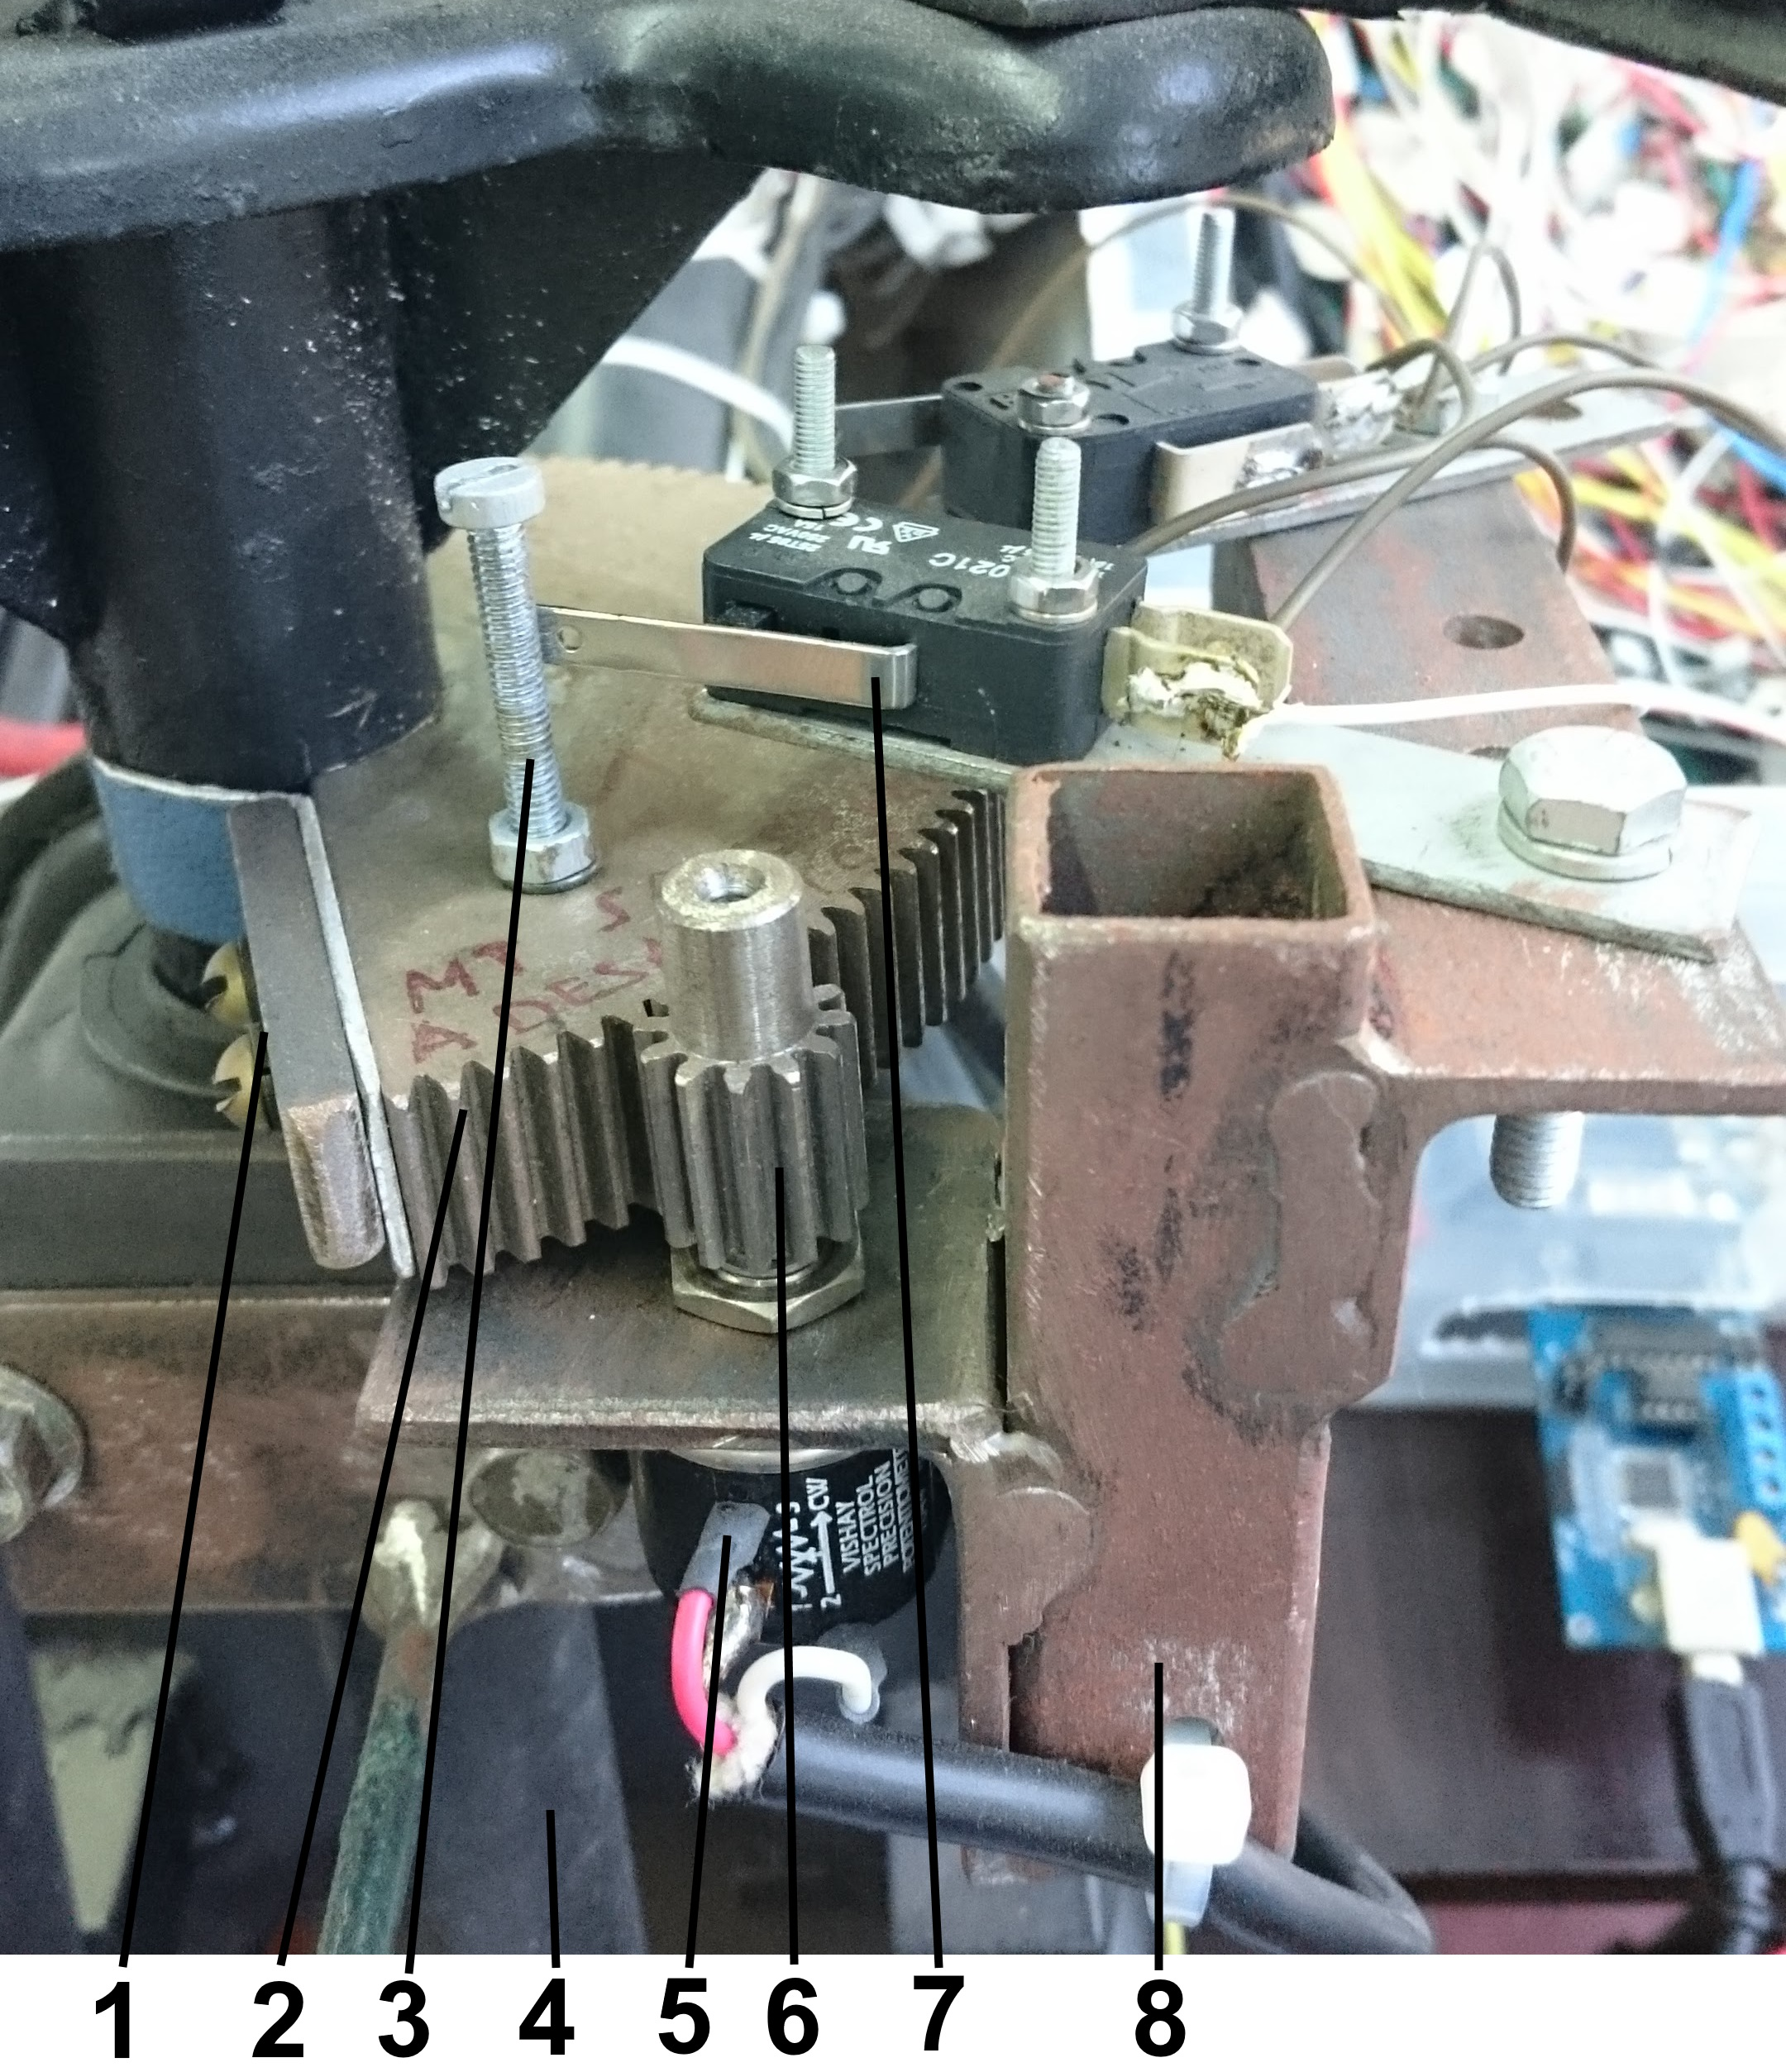
\includegraphics[width=2in]{recursos/imagens/dir_montagem_sensores.jpg} 
        \label{fig:potenciometro}}
        \caption[]{ROVIM steering subsystem's sensors and actuators.\\\hspace{\textwidth}a) steering actuator mount: 1 -- steering column; 2 -- belt tensioner; 3 -- steering column cut line, where the pulley was inserted; 4 -- steering worm drive gearbox; 5 --gearbox's output shaft; 6 -- gearbox side dented pulley; 7 -- belt; 8 -- steering motor; 9 -- steering column side dented pulley.\\\hspace{\textwidth}b) steering sensors mount: 1 -- gear column fastener; 2 -- steering column position's reading gear; 3 -- steering end of travel switch trigger; 4 -- steering column; 5 -- position reading potentiometer; 6 -- potentiometer gear; 7 -- steering end of travel switch; 8 -- sensors mount.}
\end{figure}

A potentiometer mounted near the handlebar acts as an angular position sensor, driven by a geared connection to the steering column. The same gear is used to trigger two end of travel switches (one at each side) that cut the power supply to the motor and trigger an emergency response, detailed in \ref{ssec:halt}. The set--up of the steering sensors is shown in \figurename~\ref{fig:potenciometro}.

The belt acts as a mechanical fuse, preventing damage to the set--up in case of failure, and the worm drive's unidirectional transmission characteristics act as a terrain irregularities filter. It also means that the steering cannot be driven by the handlebar while the worm drive is engaged, the user having to loosen the belt by means of the adjustable tensioner. Due to poor dimensioning, the belt slips under load (loads lower than \SI{10.25}{\newton\meter} are enough to cause it to slip), severely limiting the design of the control system. Therefore a simple proof--of--concept controller for the unloaded (wheels of the ground) setup was designed.

The microcontroller employed, discussed in more detail in \ref{ssec:integracao}, has a built--in motor position \ac{PD} control routine (the integral part is already inherent to the variable under control) that was programmed with a controller with parameters:
%
\begin{align}
    K_p &= \num{0.594}\\
    K_d &= \num{1.5}
\end{align}

\subsection{T2D's integration electronics}
\label{ssec:integracao}

To integrate the capabilities of the actuators, an array of electronic systems were deployed that, in combination with the microcontroller's running program, provide a coherent set of driving, monitoring and communication features. These electronics consist of a relay operated 2 to 1 multiplexer to choose the driving mode, a safety stop mechanism and signal conditioning circuits for the microcontroller signals, all soldered into prototype \acp{PCB}, and manual instrumentation, fastened to control panels ergonomically positioned in the vehicle. Most of these systems, along with the brake controller, the microcontroller board and the steering motor driver were wired and grouped in a plastic box, protecting them from the elements and accidental interference.

\subsubsection{Safety halt mechanism}
\label{ssec:halt}

A safety mechanism controls power delivery to the brake and traction motors in a complementary fashion, and is triggered by an array of controls, available both to a nearby user or a remote controlling computer, ensuring that in case of emergency the system is brought to a controlled halt.

It works by means of a two circuit relay array triggered by each of the possible emergency flags: a dead man trigger, an emergency switch, a signal from the microcontroller, and the end of travel switches. The dead man trigger consists of a fuse sitting on its holder in a unimpeded location, and tied with a long string that also ties to the body of the human user, when it is present, and that in case of vehicle runaway pops and triggers the emergency flag. The emergency switch consists of a standard red and yellow kill switch used in the industry, located at rear of the vehicle, for easier access. The microcontroller trigger is a dedicated output signal from the microcontroller used to trigger a monostable circuit, so that even if the software fails, only a signal pulse is needed to bring the system to a halt. The end of travel switches from the steering set--up trigger a condition when any of them is set, whereas the brake unlock side end of travel switch is used to assure binary operation of the brake, by triggering the safety mechanism when the brake is not fully unlocked.

The steering motor's power delivery is not controlled by this mechanism directly, as it does not pose such a serious threat to human lives if out of control. Nevertheless it's end of travel switches, besides triggering this safety mechanism, ensure it's power in also cut in case of a serious error.

\subsubsection{Instrumentation panels}

In order to manually control the operation of the vehicle, an array of manual controls and indicators are available. They are respectively listed in \tablename~\ref{tab:hwinputs} and \tablename~\ref{tab:leds} and shown in \figurename~\ref{fig:controlos}. These serve three main purposes: drive the vehicle, provide basic status information and control its safety mechanism.

\begin{figure}[!t]%[bhp]
    \centering
        \subfloat[]{
        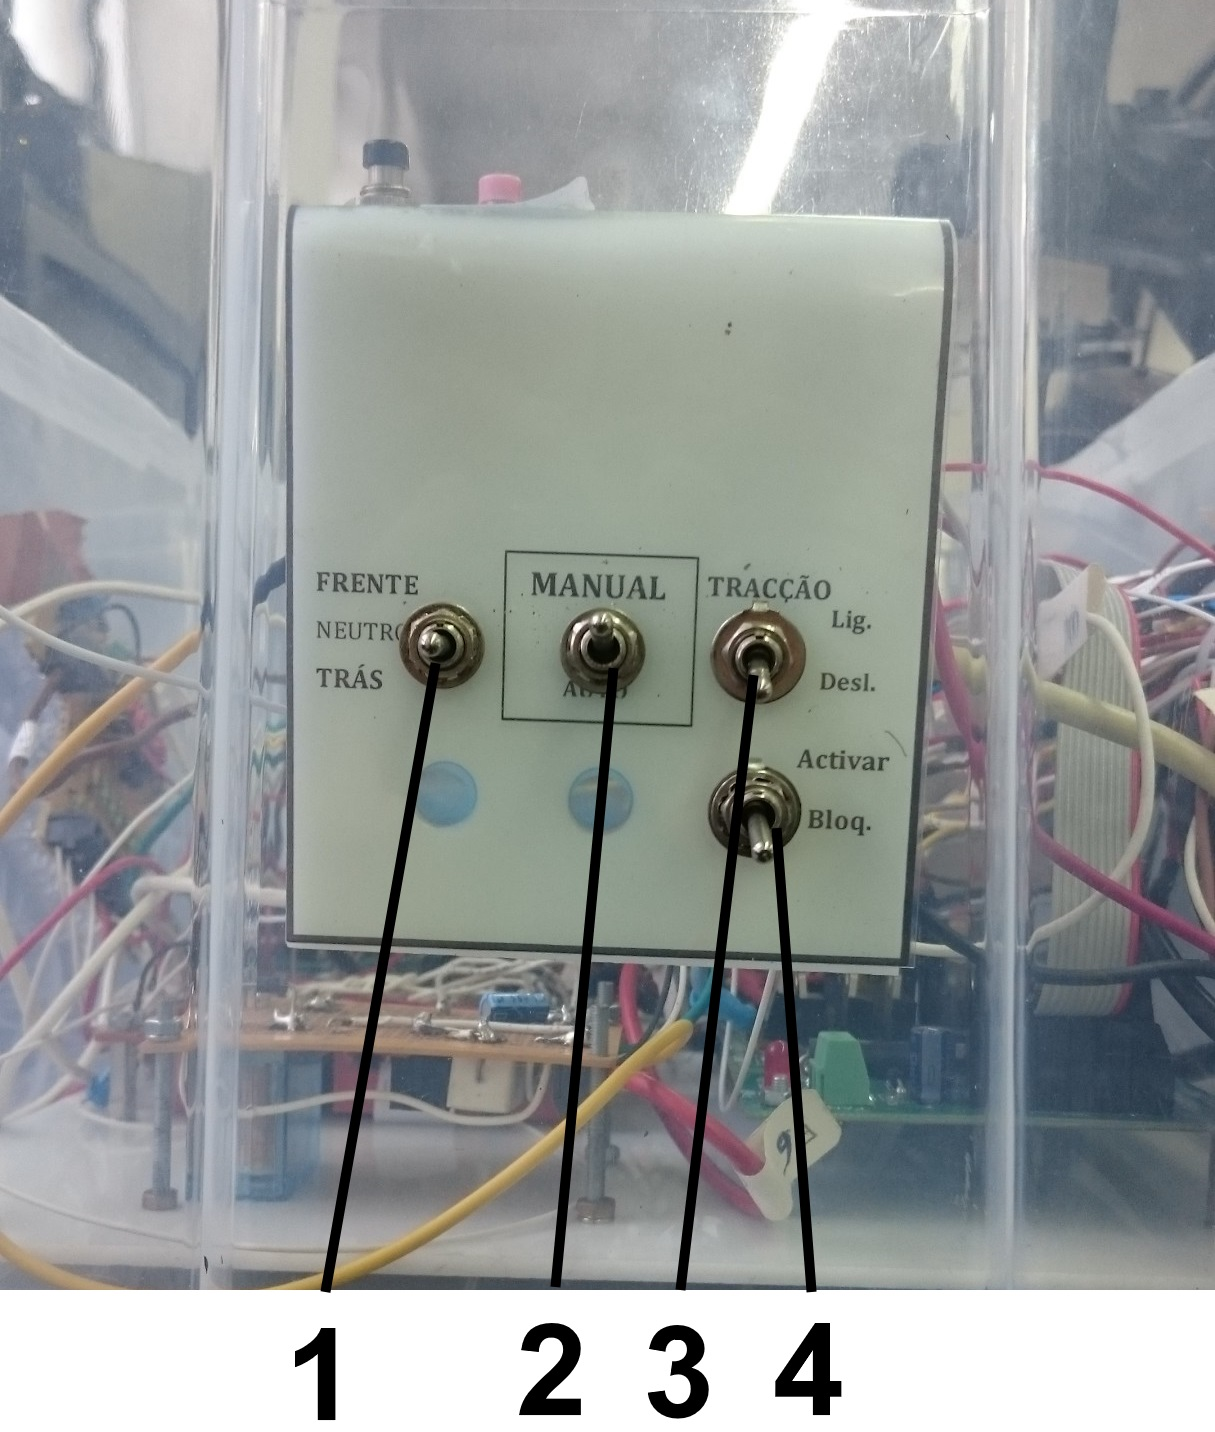
\includegraphics[width=2in]{recursos/imagens/painel_parte_acessivel.jpg} }
        \hfill
        \subfloat[]{
        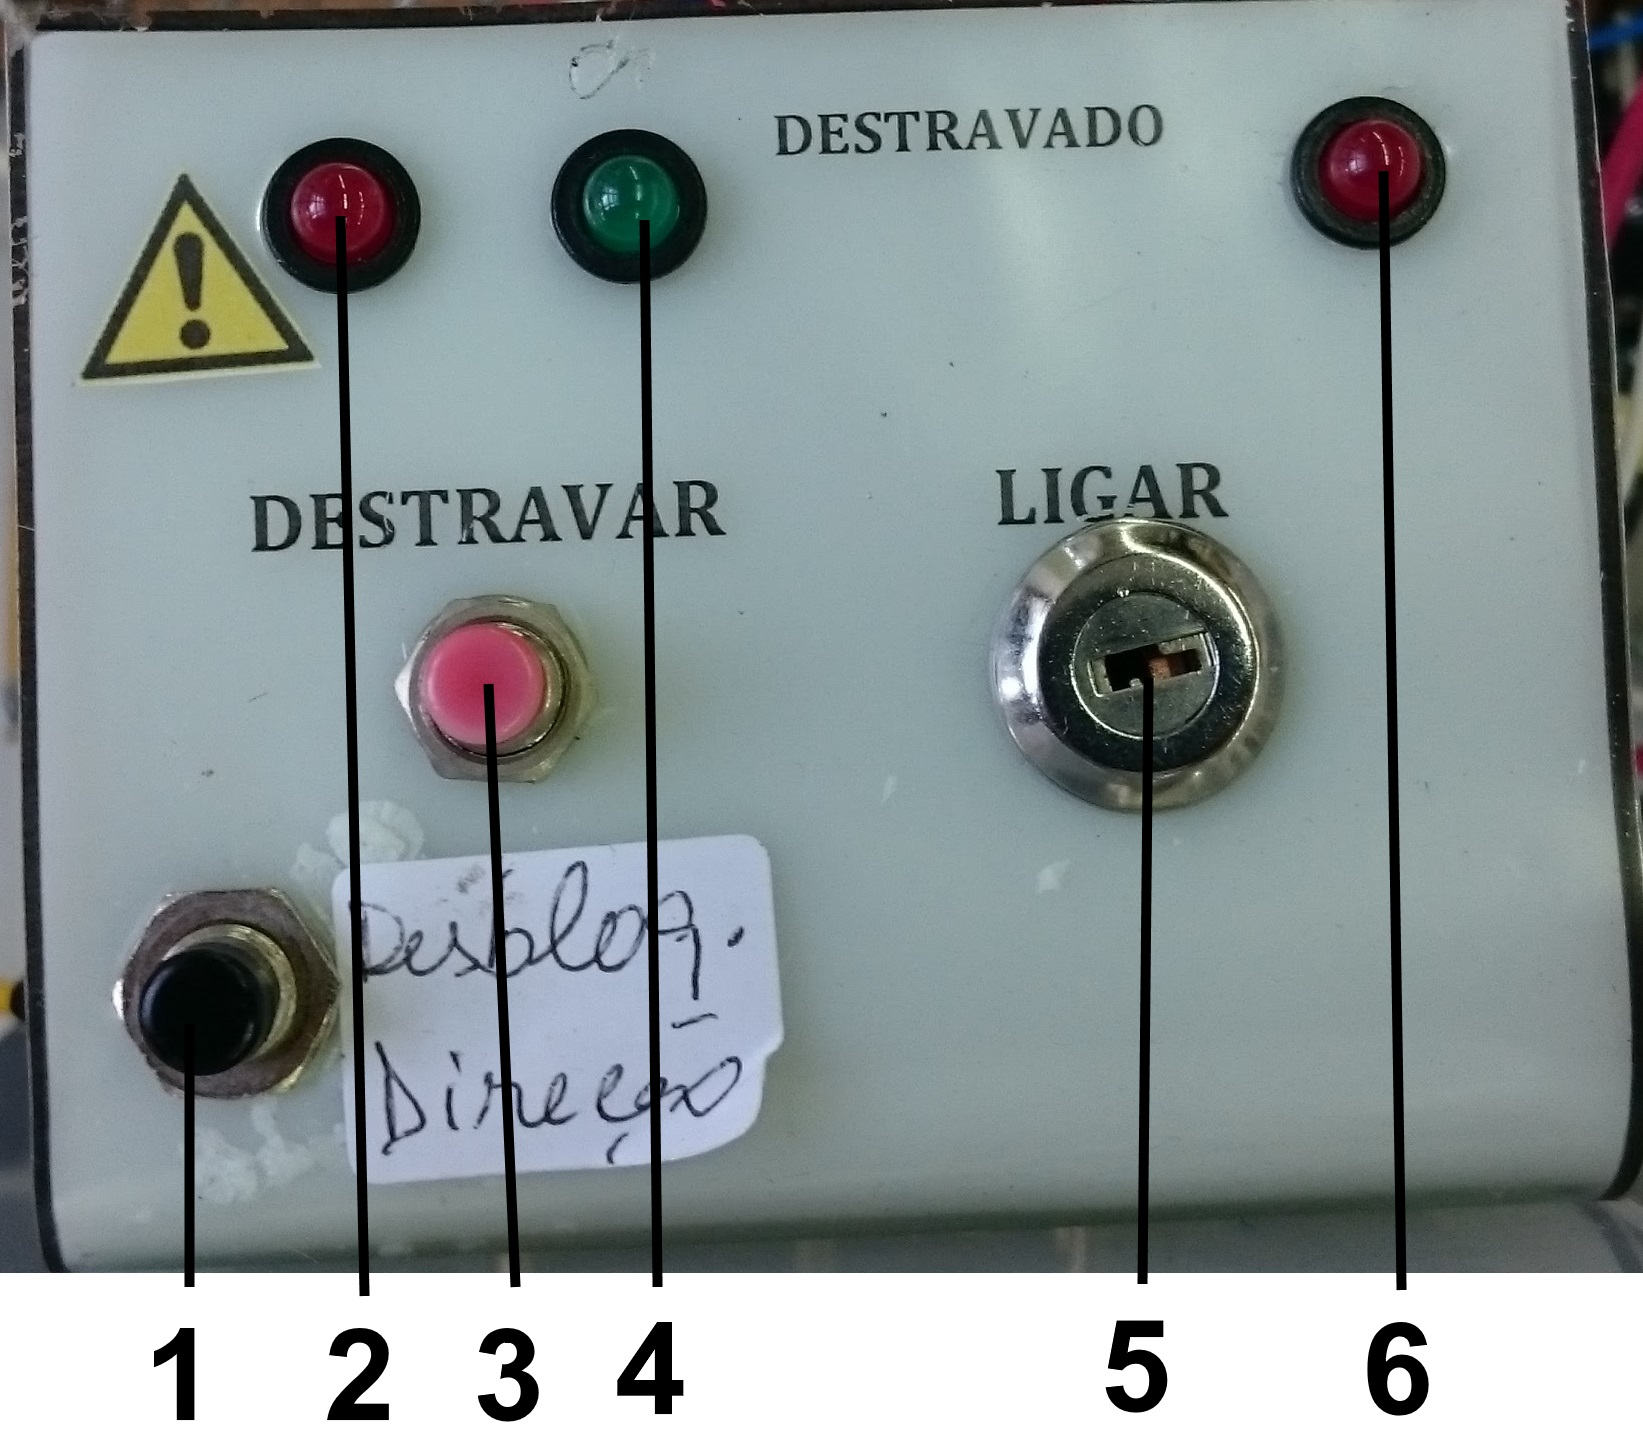
\includegraphics[width=2in]{recursos/imagens/painel_parte_protegida.jpg} }
        \hfill
        \subfloat[]{
        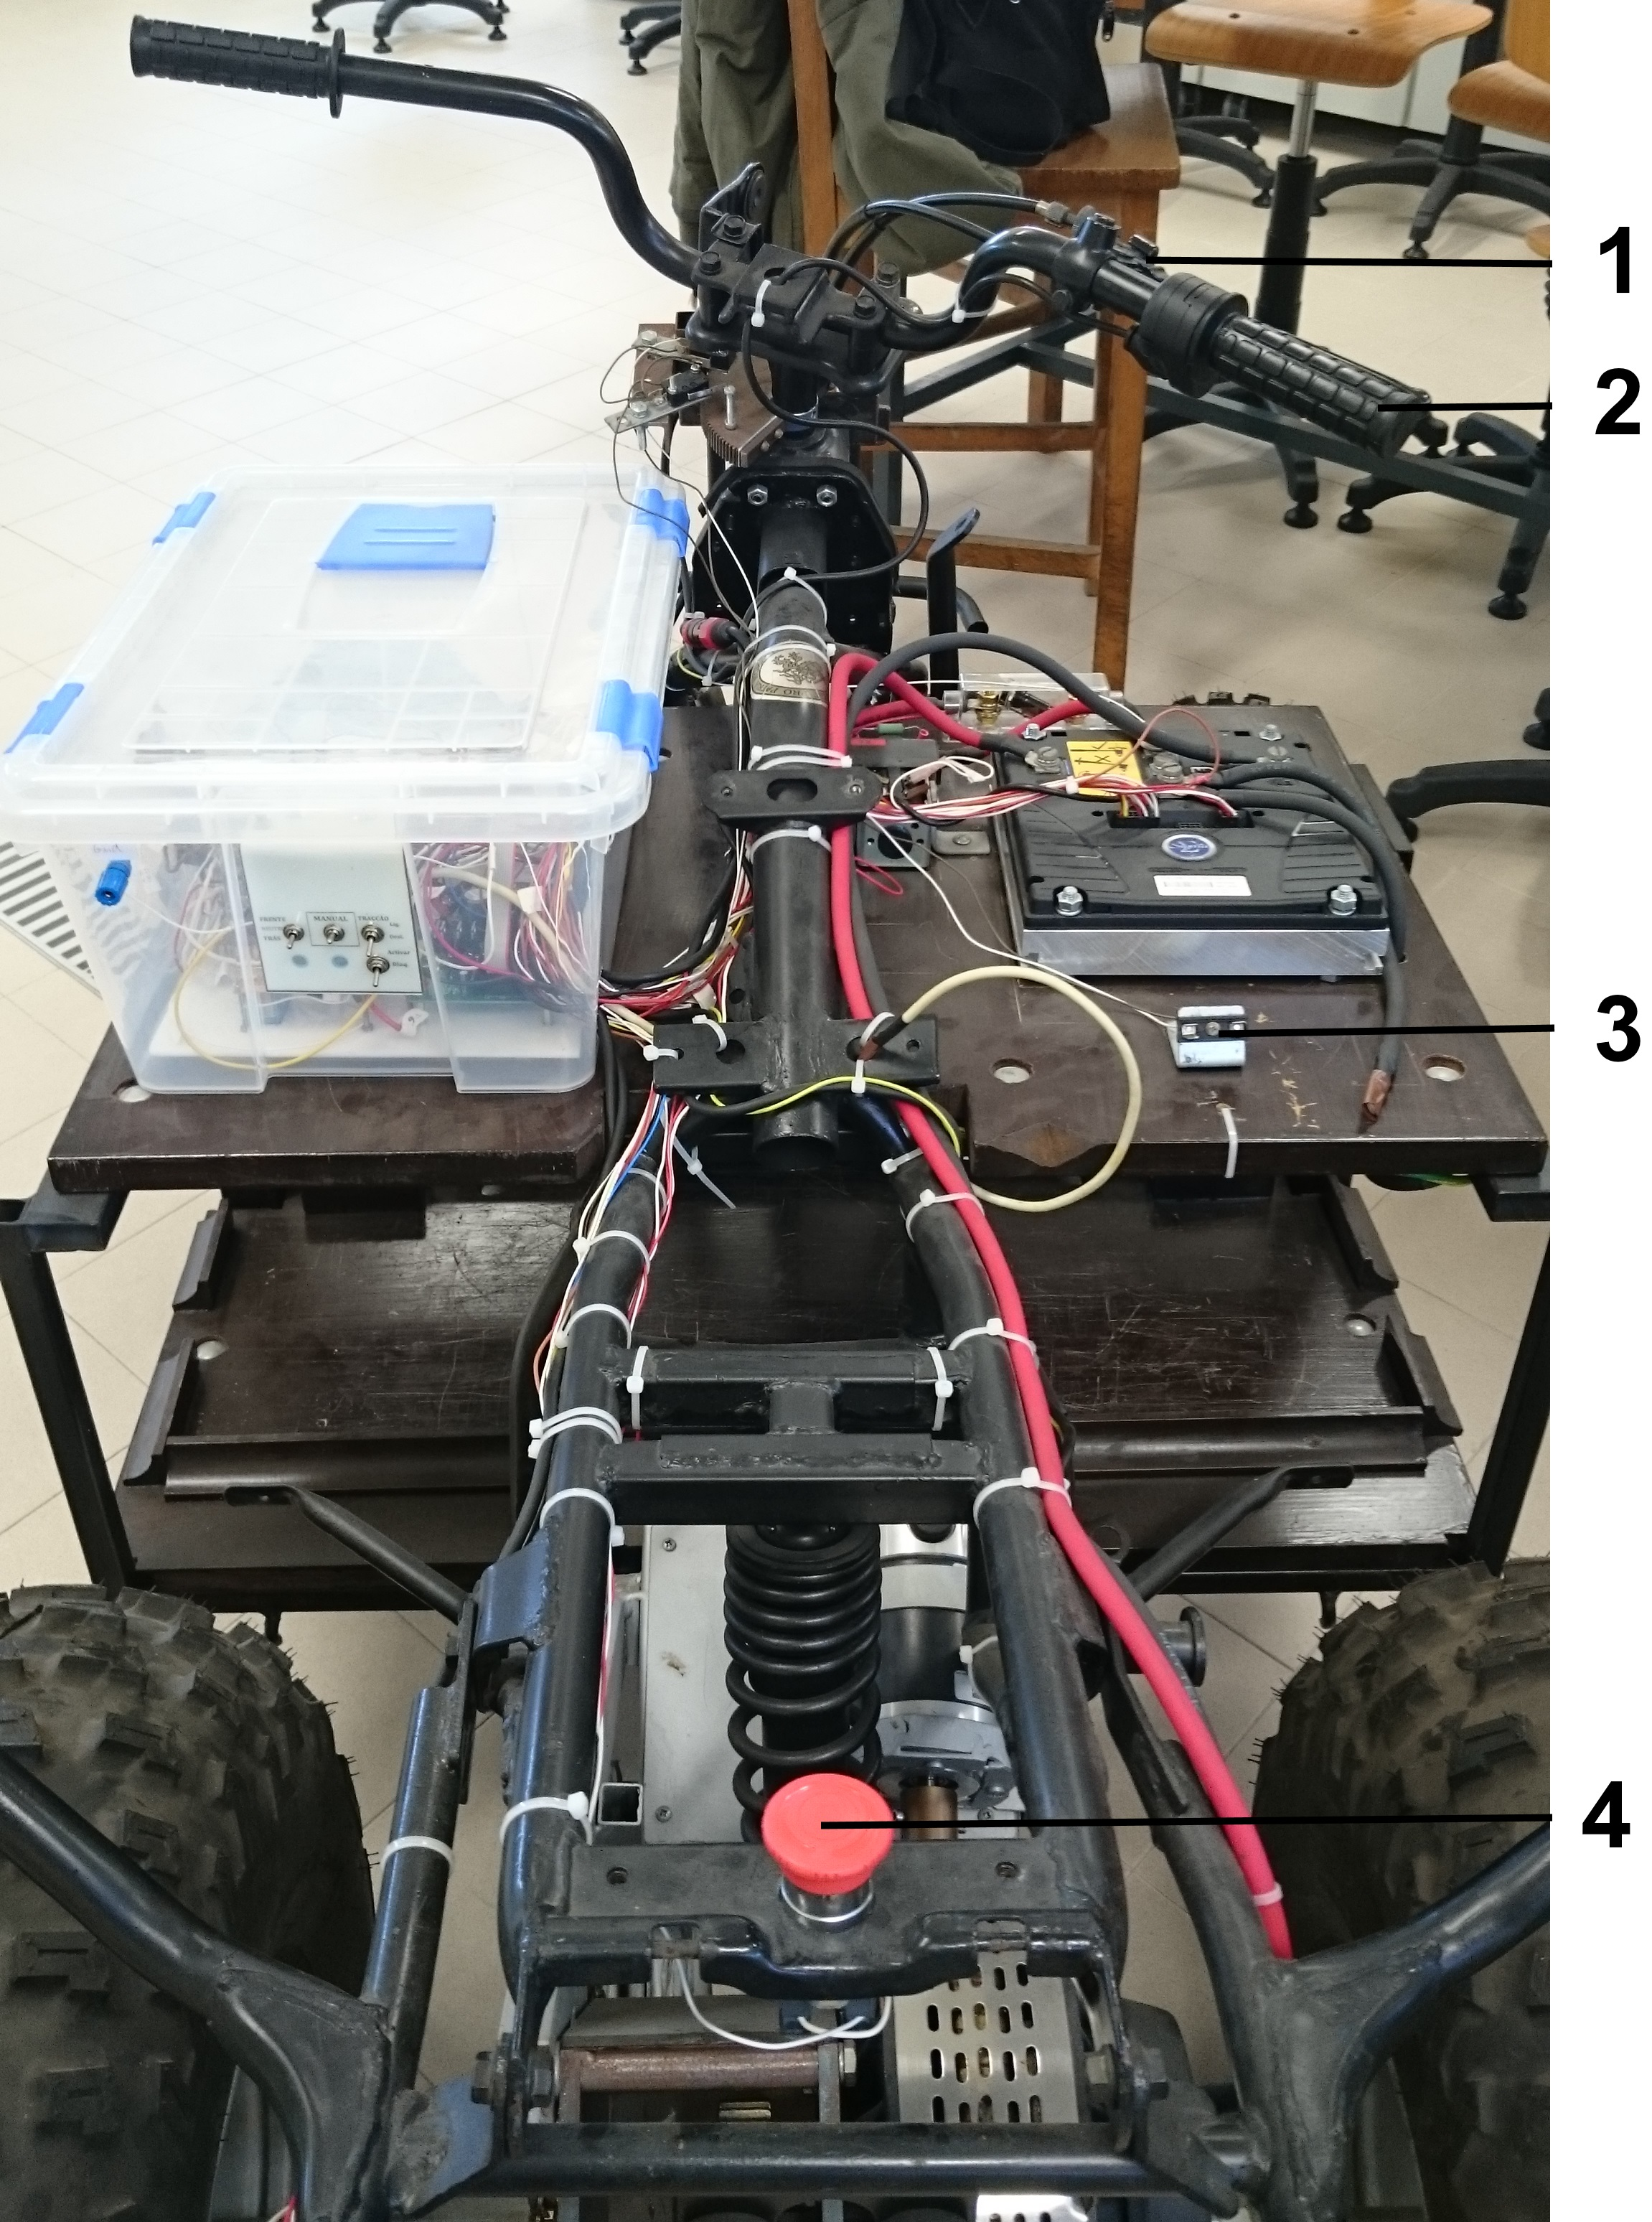
\includegraphics[width=2in]{recursos/imagens/paineis_exteriores.jpg} }
        \caption[]{ROVIM T2D's instrumentation panels.\\\hspace{\textwidth}a) 1 -- travel direction selector; 2 -- driving mode selector; 3 -- traction ON/OFF switch; 4 -- traction activation switch.\\\hspace{\textwidth}b) 1 -- steering error recovery pressure button; 2 -- brake lock indicator; 3 -- brake unlock pressure button; 4 -- brake unlock indicator; 5 -- main ON/OFF key switch; 6 -- traction error indicator.\\\hspace{\textwidth}c) 1 --front brake lever; 2 -- hand throttle; 3 -- Dead man trigger; 4 --emergency switch.}
        \label{fig:controlos}
\end{figure}

%\begin{table}[!t]
%% increase table row spacing, adjust to taste
%\renewcommand{\arraystretch}{1.3}
% if using array.sty, it might be a good idea to tweak the value of
% \extrarowheight as needed to properly center the text within the cells
%\caption{An Example of a Table}
%\label{table_example}
%\centering
%% Some packages, such as MDW tools, offer better commands for making tables
%% than the plain LaTeX2e tabular which is used here.
%\begin{tabular}{|c||c|}
%\hline
%One & Two\\
%\hline
%Three & Four\\
%\hline
%\end{tabular}
%\end{table}

\begin{table}[!t]
    \renewcommand{\arraystretch}{1.3}
    \caption{ROVIM T2D's manual controls.}
    \label{tab:hwinputs}
    \centering
    \begin{tabular} {@{} m{0.2\columnwidth} m{0.4\columnwidth} m{0.15\columnwidth} @{}}
        \hline%
        Type & Function & Possible states\\
        \hline%
        %CHAVE
        Key switch & Main switch & ON\\&&OFF\\% &
        %Ligar SigmaD
        2 way switch & Traction main switch & ON\\&&OFF\\
        %M/A
        2 way switch & Drive mode selector & Manual\\&&Auto\\
        %F/N/T
        3 way switch & Select travel direction \footnotemark[1]& Front\\&&Neutral\\&&Reverse\\
        %Ativar tração
        2 way switch & Traction activation switch \footnotemark[1]& Activate\\&&Block\\
        %Destravar
        Pressure button & Unlocks electric brake & Pressed\\&&Released\\
        %Desbloquear direção
        Pressure button & Allows steering to be moved in lockdown mode & Pressed\\&&Released\\
        %Botão emergência
        Emergency switch & Triggers the safety mechanism & Pressed\\&&Released\\ 
        %Dispositivo homem morto
        Dead man trigger & Triggers the safety mechanism & Alive\\&&Dead\\
        %Acelerador
        Hand throttle & Controls vehicle speed \footnotemark[1]& \\
        %Travão de mão
        Brake lever & Brakes the front wheels &\\
        % Esticador da correia
        Belt tensioner & Engages the steering actuator & Fastened\\&&Loose\\ 
        %Botão dalf reiniciar
        Pressure button & Reboots the microcontroller & Pressed\\&&Released\\
        \hline
    \end{tabular}%
\end{table}


\begin{table}[!t]
    \renewcommand{\arraystretch}{1.3}
    \caption{ROVIM T2D's LEDs}
    \label{tab:leds}
    \centering
    \begin{tabular} {@{} m{0.2\columnwidth} m{0.15\columnwidth} m{0.4\columnwidth} @{}}
        \hline%
        Name & Colours & Indicates\\
        \hline%
        Brake unlock & Green & Brake fully unlocked \footnotemark[2]\\
        Brake lock & Red & Brake not fully unlocked\\
        Traction error & Red & Traction motor controller error \\
        Control panel traction error & Red & Same as "Traction error" \ac{LED}\\
        Traction presence & Green & Traction motor controller is ON\\
        Direction presence & Green & Steering motor driver is ON\\
        Microcontroller presence & Green & Microcontroller is ON\\
        MTR1 & Green & Direction and duty cycle of traction motor \footnotemark[3]\\
             & Red\\
        MTR2 & Green & Direction and duty cycle of steering motor \footnotemark[3]\\
             & Red\\
        LED1 & Green & Traction motor state \footnotemark[3]\\
        LED2 & Green & Steering motor state \footnotemark[3]\\
        LED3 & Red & System error\\
        Travel blink & Red & Vehicle is moving\\
        \hline
    \end{tabular}
\end{table}

\subsubsection{Microcontroller signal conditioning}

\footnotetext[1]{When on manual driving mode.}
\footnotetext[2]{Only when the brake unlock pressure button is being pressed.}
\footnotetext[3]{When on autonomous driving mode.}
Most signals read by the microcontroller are connected to mechanical switches operating at \SI{12}{\volt} and have to be converted to the \SI{5}{\volt} logic of the microcontroller and debounced. This task is performed by a simple resistive voltage divider and low pass $RC$ filter. The voltage divider consists of an upper \SI{74}{\kilo\ohm} resistor in series with a ground connected \SI{47}{\kilo\ohm} one, ensuring that for the worst case scenario (a new, fully charged battery with a $\approx\SI{14}{\volt}$ output) the divided voltage remains within the input tolerance of the \ac{IC}. A ground connected \SI{0.1}{uF} capacitor performs a low pass filter with the \SI{28.7}{\kilo\ohm} voltage divider equivalent resistor, with $\approx\SI{50}{\hertz}$ cut-off frequency, which is enough to filter switch bouncing and provide accurate readings for the microcontroller. The graphics in \figurename~\ref{fig:debouncer} show the performance of the circuit. To limit the maximum input voltage to the \ac{IC}, a clipping diode was connected from the input pin to the circuit's supply.% Two resistors in series were used for the high side of the voltage divider consists of two series resistors instead of only one, to maintain operation when one of them fails and becomes a short circuit.

The traction motor controller expects an analogue signal for both its accelerator and regenerative braking control inputs. To provide that kind of signal, the microcontroller outputs a \SI{10}{\hertz} \ac{PWM} signal from a digital output pin that is converted to analogue by a low pass $RC$ filter with a cut-off frequency of \SI{1}{\hertz}. The output analogue signal presents a peak to peak ripple of $\approx\SI{30}{\%}$ that shows no hiccups on the output speed because the traction controller is programmed to accelerate very slowly.

\begin{figure}
    \centering
        \subfloat[]{
        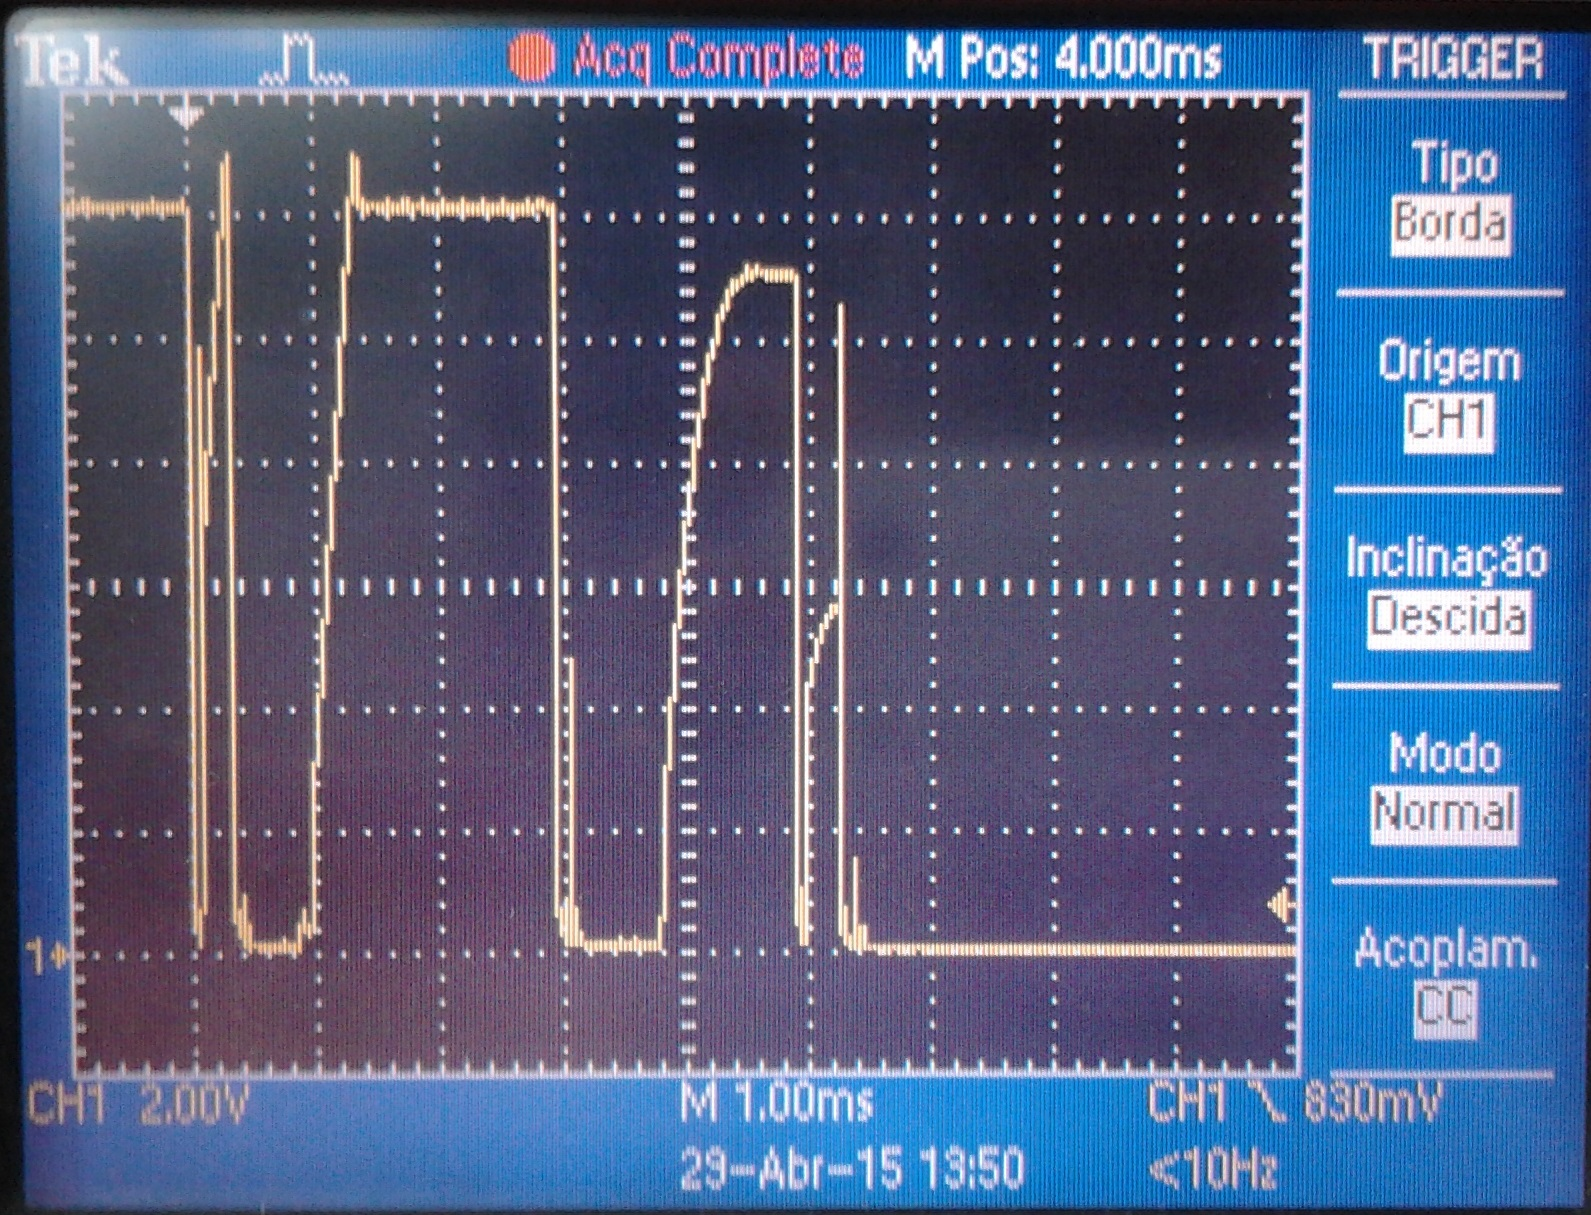
\includegraphics[width=2in]{recursos/imagens/comutacao_int_alavanca.jpg} }
        \hfill
        \subfloat[]{
        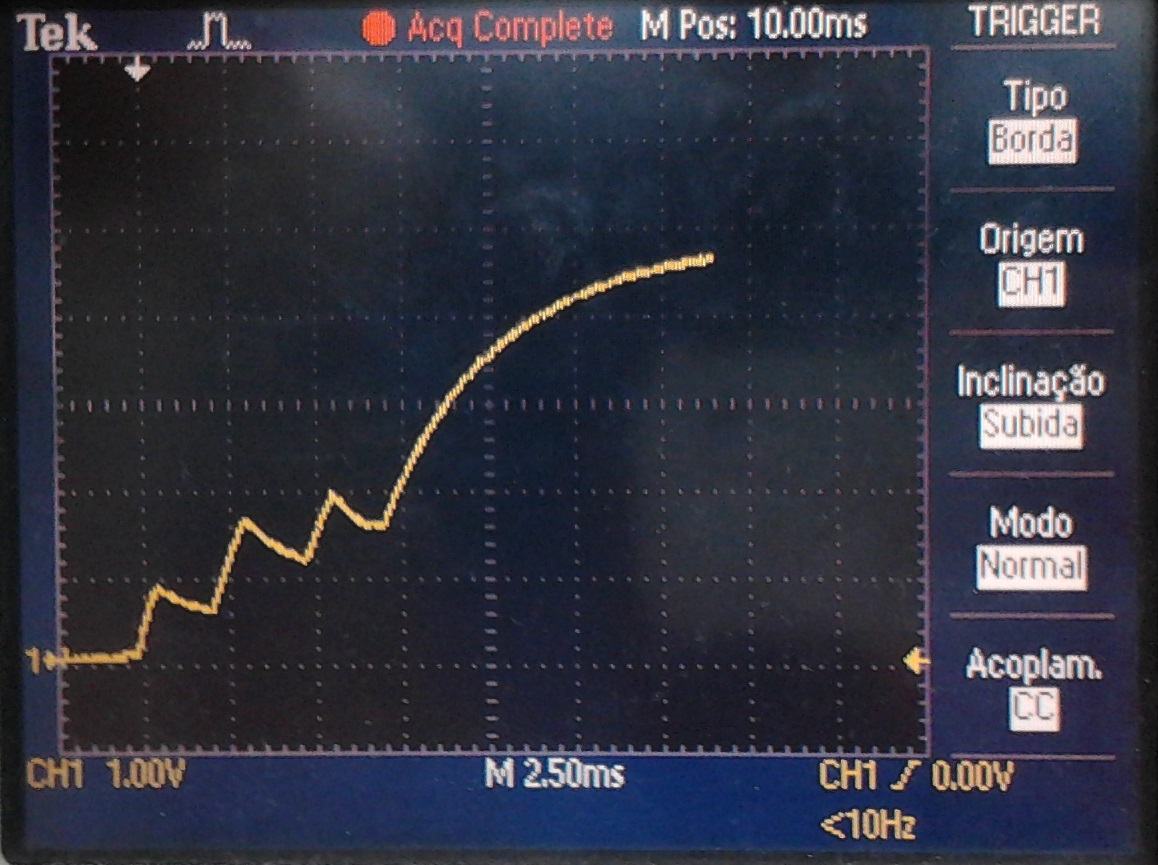
\includegraphics[width=2in]{recursos/imagens/comutacao_filtrada.jpg} }
        \caption[]{ROVIM T2D's microcontroller's input signal conditioning results.\\\hspace{\textwidth}a) mechanical switch bounce. Y axis is switch voltage at \SI{2}{\volt/div}; X axis is time at \SI{1}{\milli\second/div}.\\\hspace{\textwidth}b) filtered and voltage converted switch bounce. Y axis is IC input pin's voltage at \SI{1}{\volt/div}; X axis is time at \SI{2.5}{\milli\second/div}.}
        \label{fig:debouncer}
\end{figure}


\subsection{Control program}

To provide autonomous driving and system wide monitoring capabilities, a control program was developed by extending the original firmware provided with the microcontroller board acquired. The original is an interrupt--driven, dual motor control program, with an \ac{ASCII} formatted serial port command interface geared towards human users and an \ac{I2C} in slave mode binary interface, geared towards control by other computers \cite{dalf_om}. The firmware uses almost all hardware resources already, but still was extended, with little loss of original functionality, to control the traction motor controller, trigger the safety mechanism, monitor the sensors in the system and provide an interface to access all these features.

To do so, the hardware signals listed on the \tablename~\ref{tab:sinais_uc} were routed to the microcontroller board, to provide a means to deploy the new capabilities. On the software, besides extending the interrupt driven command dispatcher, two periodic tasks were created, one providing \ac{PWM} signals to the traction accelerator and decelerator, and the other monitoring the system and performing delayed actions. The actions performed by the monitoring task are listed on \tablename~\ref{tab:acoes_monitor_system}.

The control of the steering position was implemented using the \ac{PID} motor control routine of the original firmware, that controls the steering motor driver through it's specific interface. On top of it, a custom function was built to abstract the user from the machine representation of the angular position and the misalignment between the sensor's mid course position and the steering's. The user now only has to specify the desired angular position of the wheels, knowing the angular position's representation: \SI{86}{\degree} being a full starboard turn, \SI{0}{\degree} being a full port turn, and its midpoint, \SI{43}{\degree}, now being the direction's mid position.

Acceleration and deceleration controls and a open loop vehicle movement control command were also developed. The movement command allows one of four movement types to be selected: forward, reverse, neutral and immobilization. In order to provide speed readings, the original quadrature encoder reading interrupt had to be adapted to the single source sensor used here, by connecting the quadrature signal input to ground and recalibrating the interrupt.

To mitigate possible software failures, the watchdog was activated, and since the microcontroller's reset signal could not be sourced from the board, the start-up sequence triggers the safety mechanism as early as possible. When it detects or triggers the safety mechanism's activation, the software responds accordingly by forbidding all motor movement and actions not strictly needed to recover from the error detected, what is called the lockdown state. To be able to move the vehicle (either manually or by software), the user has to solve any underlying error conditions and deliberately unlock the brake in coordination with the software. Besides providing a high safety standard, this procedure ensures that the vehicle always starts at a known state.

Besides having new commands added, the serial interface was also modified to provide a much more verbose interaction with the user, making novice users's interaction with the program easier. For the advanced user, real time software debug and control features added during the software development stage remain available in the field versions.

\begin{table}[!t]

    \renewcommand{\arraystretch}{1.3}
        \caption{Microcontroller's input and output signals.}
        \label{tab:sinais_uc}
    \centering
    \begin{tabular}{@{}  m{0.25\columnwidth} m{0.15\columnwidth} m{0.45\columnwidth}  @{}}
            \hline
            Name & Polarity & Function\\
            \hline
            Decelerator & Output & Controls regenerative braking \footnotemark[3]\\
            Brake unlocked & Input & Detect brake fully unlocked\\
            Accelerator & Output & Controls traction acceleration \footnotemark[3]\\
            B+ & Input & Detects traction controller being powered\\
            Activate Traction & Output & Controls the traction activation switch \footnotemark[3]\\
            Brake locked & Input & Detects brake fully locked\\
            Unlock brake & Output & Unlocks the brake \footnotemark[4]\\
            Steering error & Input & Detects steering out of bounds\\
            Reverse & Output & Selects reverse travel direction \footnotemark[3]\\
            Manual unlock & Input & Detects brake being unlocked by the user\\
            Forward & Output & Selects forward travel direction \footnotemark[3]\\
            Manual mode & Input & Detects manual driving mode selected\\
            Lock & Output & Locks the brake\\
            Emergency & Input & Emergency state detected\\
            Handbrake & Output & Imobilizes the vehicle \footnotemark[3]\\
            Position & Input & Measure direction's angular position\\
            Speed & Input & Measure vehicle speed\\
            \hline
        \end{tabular}

\end{table}

\footnotetext[4]{Currently the pin is not connected.}

\begin{table}[!t]

    \renewcommand{\arraystretch}{1.3}
        \caption{Actions of the monitoring task.}
        \label{tab:acoes_monitor_system}
        \centering
        \begin{tabular}{@{} m{0.33\columnwidth} m{0.25\columnwidth} m{0.33\columnwidth}  @{}}
            \hline
            Condition & Actions taken & Motive\\
            \hline
            Speed too high & Goes to lockdown & Slow down the vehicle\\
            Vehicle immobilized and moving \footnotemark[3] & Goes to lockdown & Incoherent state\\
            Emergency state detected \footnotemark[5] & Goes to lockdown & Assure consistency with hardware state\\
            Electric brake neither locked nor unlocked & Goes to lockdown & Enforce binary braking action\\
            Direction end of travel triggered & Goes to lockdown & Assure consistency with hardware state\\
            Taking too long to unlock brake & Goes to lockdown & Precaution \\
            Manual driving mode selected & Stops motors & Avoid unexpected motor movement when reverting to auto mode\\
            \hline
        \end{tabular}

\end{table}

\footnotetext[5]{The safety mechanism has been triggered.}

\begin{table}[!t]

    \renewcommand{\arraystretch}{1.3}
        \caption{Useful commands to operate the ROVIM.}
        \label{tab:comandos_rovim}
        \centering
        \begin{tabular}{@{} m{0.1\columnwidth} m{0.25\columnwidth} m{0.45\columnwidth} @{}}
            \hline
            Command & Description & Syntax\\
            \hline
            \texttt{G10} & Go to lockdown & \texttt{G10}\\
            \texttt{G11} & Exit lockdown & \texttt{G11}\\
            \texttt{G12} & Stop motors, keep configuration & \texttt{G12 <mtr\#>}\\
            \texttt{G13} & Control GPIOs & \texttt{G13 <opção><gpio\#>}\\
            \texttt{G14} & Accelerate & \texttt{G14 <\%>}\\
            \texttt{G15} & Decelerate & \texttt{G15 <\%>}\\
            \texttt{G16} & Select movement & \texttt{G16 <dir><vel>}\\
            \texttt{G17} & Turn & \texttt{G17 <ang>}\\
            \texttt{G18} & Debug control & \texttt{G18 <op><val1><val2><val3>}\\
            \texttt{H} & Help & \texttt{H}\\
            \hline
            \texttt{O} & Stop motors, lose configuration & \texttt{O <mtr\#>}\\
            \texttt{X} & Drive motor in open loop & \texttt{X <mtr\#> <dir><\%>}\\
            \hline
        \end{tabular}

\end{table}

% An example of a floating figure using the graphicx package.
% Note that \label must occur AFTER (or within) \caption.
% For figures, \caption should occur after the \includegraphics.
% Note that IEEEtran v1.7 and later has special internal code that
% is designed to preserve the operation of \label within \caption
% even when the captionsoff option is in effect. However, because
% of issues like this, it may be the safest practice to put all your
% \label just after \caption rather than within \caption{}.
%
% Reminder: the "draftcls" or "draftclsnofoot", not "draft", class
% option should be used if it is desired that the figures are to be
% displayed while in draft mode.
%
%\begin{figure}[!t]
%\centering
%\includegraphics[width=2.5in]{myfigure}
% where an .eps filename suffix will be assumed under latex, 
% and a .pdf suffix will be assumed for pdflatex; or what has been declared
% via \DeclareGraphicsExtensions.
%\caption{Simulation results for the network.}
%\label{fig_sim}
%\end{figure}

% Note that the IEEE typically puts floats only at the top, even when this
% results in a large percentage of a column being occupied by floats.


% An example of a double column floating figure using two subfigures.
% (The subfig.sty package must be loaded for this to work.)
% The subfigure \label commands are set within each subfloat command,
% and the \label for the overall figure must come after \caption.
% \hfil is used as a separator to get equal spacing.
% Watch out that the combined width of all the subfigures on a 
% line do not exceed the text width or a line break will occur.
%
%\begin{figure*}[!t]
%\centering
%\subfloat[Case I]{\includegraphics[width=2.5in]{box}%
%\label{fig_first_case}}
%\hfil
%\subfloat[Case II]{\includegraphics[width=2.5in]{box}%
%\label{fig_second_case}}
%\caption{Simulation results for the network.}
%\label{fig_sim}
%\end{figure*}
%
% Note that often IEEE papers with subfigures do not employ subfigure
% captions (using the optional argument to \subfloat[]), but instead will
% reference/describe all of them (a), (b), etc., within the main caption.
% Be aware that for subfig.sty to generate the (a), (b), etc., subfigure
% labels, the optional argument to \subfloat must be present. If a
% subcaption is not desired, just leave its contents blank,
% e.g., \subfloat[].


% An example of a floating table. Note that, for IEEE style tables, the
% \caption command should come BEFORE the table and, given that table
% captions serve much like titles, are usually capitalized except for words
% such as a, an, and, as, at, but, by, for, in, nor, of, on, or, the, to
% and up, which are usually not capitalized unless they are the first or
% last word of the caption. Table text will default to \footnotesize as
% the IEEE normally uses this smaller font for tables.
% The \label must come after \caption as always.
%
%\begin{table}[!t]
%% increase table row spacing, adjust to taste
%\renewcommand{\arraystretch}{1.3}
% if using array.sty, it might be a good idea to tweak the value of
% \extrarowheight as needed to properly center the text within the cells
%\caption{An Example of a Table}
%\label{table_example}
%\centering
%% Some packages, such as MDW tools, offer better commands for making tables
%% than the plain LaTeX2e tabular which is used here.
%\begin{tabular}{|c||c|}
%\hline
%One & Two\\
%\hline
%Three & Four\\
%\hline
%\end{tabular}
%\end{table}


% Note that the IEEE does not put floats in the very first column
% - or typically anywhere on the first page for that matter. Also,
% in-text middle ("here") positioning is typically not used, but it
% is allowed and encouraged for Computer Society conferences (but
% not Computer Society journals). Most IEEE journals/conferences use
% top floats exclusively. 
% Note that, LaTeX2e, unlike IEEE journals/conferences, places
% footnotes above bottom floats. This can be corrected via the
% \fnbelowfloat command of the stfloats package.



\section{Conclusion}

The main goal of this project, to build a functioning prototype of an autonomous, electric vehicle was achieved. Personnel safety was at the forefront of design concerns, and a robust and reliable safety halt mechanism was built, with multiple triggers. Clever packaging allowed a neat component separation, and a hidden battery rack.

However, limitations in fabrication methods meant that contact are still unprotected and batteries loose, posing a potential safety threat. Also, failure to build an effective mechanical coupler to the wheels resulted in limited use capabilities for the vehicle.

Access to more advanced battery fixing capabilities, such as auto industry mounts and contact protections, and a steering transmission refitting can solve both problems and achieve a very robust vehicle, with a lot of potential to unlock.





% if have a single appendix:
%\appendix[Proof of the Zonklar Equations]
% or
%\appendix  % for no appendix heading
% do not use \section anymore after \appendix, only \section*
% is possibly needed

% use appendices with more than one appendix
% then use \section to start each appendix
% you must declare a \section before using any
% \subsection or using \label (\appendices by itself
% starts a section numbered zero.)
%


\appendix[Program code]
An exact copy of the code files of the microcontroller program is available at: \url{https://github.com/ROVIM-T2D/ROVIM-T2D-Brain/tree/v1.0}.

% you can choose not to have a title for an appendix
% if you want by leaving the argument blank
%\section{Electrical circuits schematics}
%Don't know how to include them


% use section* for acknowledgment
\section*{Acknowledgment}

This project was funded by Academia Militar, a Portuguese public military higher education institution, 1169-203 Lisbon, Portugal. E-mail: (see http://academiamilitar.pt/).


%The authors would like to thank...


% Can use something like this to put references on a page
% by themselves when using endfloat and the captionsoff option.
\ifCLASSOPTIONcaptionsoff
  \newpage
\fi



% trigger a \newpage just before the given reference
% number - used to balance the columns on the last page
% adjust value as needed - may need to be readjusted if
% the document is modified later
%\IEEEtriggeratref{8}
% The "triggered" command can be changed if desired:
%\IEEEtriggercmd{\enlargethispage{-5in}}

% references section

% can use a bibliography generated by BibTeX as a .bbl file
% BibTeX documentation can be easily obtained at:
% http://mirror.ctan.org/biblio/bibtex/contrib/doc/
% The IEEEtran BibTeX style support page is at:
% http://www.michaelshell.org/tex/ieeetran/bibtex/
\bibliographystyle{IEEEtran}
% argument is your BibTeX string definitions and bibliography database(s)
\bibliography{IEEEabrv,recursos/biblio.bib}
%
% <OR> manually copy in the resultant .bbl file
% set second argument of \begin to the number of references
% (used to reserve space for the reference number labels box)
%\begin{thebibliography}{1}
%
%\bibitem{IEEEhowto:kopka}
%H.~Kopka and P.~W. Daly, \emph{A Guide to \LaTeX}, 3rd~ed.\hskip 1em plus
%  0.5em minus 0.4em\relax Harlow, England: Addison-Wesley, 1999.
%
%\end{thebibliography}

% biography section
% 
% If you have an EPS/PDF photo (graphicx package needed) extra braces are
% needed around the contents of the optional argument to biography to prevent
% the LaTeX parser from getting confused when it sees the complicated
% \includegraphics command within an optional argument. (You could create
% your own custom macro containing the \includegraphics command to make things
% simpler here.)
%\begin{IEEEbiography}[{\includegraphics[width=1in,height=1.25in,clip,keepaspectratio]{mshell}}]{Michael Shell}
% or if you just want to reserve a space for a photo:

%\begin{IEEEbiography}{Gon\c{c}alo Andr\'e}
%    Gon\c{c}alo Andr\'e is a student of Electrotechnic and Computer Engineering at Instituto Superior T\'ecnico, in Lisbon.
%\end{IEEEbiography}

% if you will not have a photo at all:
\begin{IEEEbiographynophoto}{Gon\c{c}alo F. R. Andr\'e}
    is currently a MSc student of Electrotechnic and Computer Engineering at Instituto Superior T\'ecnico, in Lisbon.
\end{IEEEbiographynophoto}
%
%% insert where needed to balance the two columns on the last page with
%% biographies
%%\newpage
%
%\begin{IEEEbiographynophoto}{Jane Doe}
%Biography text here.
%\end{IEEEbiographynophoto}

% You can push biographies down or up by placing
% a \vfill before or after them. The appropriate
% use of \vfill depends on what kind of text is
% on the last page and whether or not the columns
% are being equalized.

%\vfill

% Can be used to pull up biographies so that the bottom of the last one
% is flush with the other column.
%\enlargethispage{-5in}

% that's all folks
\end{document}


